\section{Learning Sequential Structure From State Demonstrations}
DDO is an inference algorithm that applies to the supervised demonstration setting where state-action tuples are available. Next, we explored algorithms for leveraging state-demonstrations for structuring RL exploration.
Like DDO, we apply unsupervised learning to a small number of initial expert demonstrations to structure future autonomous exploration. Leveraging what we can learn from a small dataset of state-demonstrations, instead of decomposing a task into a hierarchy of controllers, we decompose it into a hierarchy of waypoints. First, I present our inference algorithm for learning waypoint structure from state demonstrations. Then, I describe how we incorporated these waypoints into a planner.

\subsection*{Introduction}
While one could infer such criteria from manual annotations or matching to pre-defined dictionaries of motion templates, labeling consistency and supervisory burden are a concern in \emph{supervised} approaches.
Complex, high-dimensional data can require a large amount of labels before a viable segmentation model can be learned.
Similarly, dictionaries of primitives can be incomplete.
To avoid these problems, \emph{unsupervised} segmentation methods have been long studied ~\cite{viviani1985segmentation,morasso1983three,sternad1999segmentation}.
Recently, there are several new probabilistic approaches that pose segmentation as a probabilistic inference problem~\cite{barbivc2004segmenting, chiappa2010movement,  alvarez2010switched,kruger2012imitation, niekum2012learning, wachter2015hierarchical}.
The approaches model a trajectory as generated from a mixture of parametrized dynamical regimes, and an inference procedure learns the dynamical parameters--which can be used to identify time segments at which each regime is active.

Explicitly modeling the dynamics can require learning a large number of parameters.
This makes such approaches somewhat sensitive to any noise in the dataset, especially when the datasets are small. 
This sensitivity leads to challenges in applications like robotic surgery.
The adoption of robot-assisted minimally invasive surgery (RMIS)  generating datasets of kinematic and video recordings of surgical procedures~\cite{gao2014jigsaws}, and where trajectories are collected from teleoperation interfaces.
With such interfaces, we have observed significant jitter in motion and noise due to time delays~\cite{chuck2017statistical, liangusing}.
Figure \ref{teaser} plots 10 expert demonstrations of a surgical training task.
In such a setting, the robustness and stability of the segmentation algorithm are a key concern in surgical segmentation, and to the best of our knowledge, prior work mitigates this issue by leveraging pre-defined dictionaries of motion segments~\cite{lin2006towards, lin2005automatic}.

In many important tasks, while the demonstration motions may vary and be noisy, each demonstration contains roughly the same order of true segments, e.g., well-defined surgical training procedures.
This consistent, repeated structure can be exploited to infer global segmentation criteria.
By assuming known sequential segment-to-segment transitions, the problem reduces to identifying a common set of segment-to-segment transition events--not corresponding entire the trajectory segments across the whole dataset.
This allows us to apply coarser, imperfect motion-based segmentation algorithms first that create a large set of candidate transitions.
Then, we can filter this set by identifying transition events that occurred at similar times and states.
Our experiments suggest that this approach has improved robustness and sample-efficiency, while approximating the behavior of more complicated dynamical systems-based approaches in many real problems.

I formalize this intuition into a new hierarchical clustering algorithm for unsupervised segmentation called Transition State Clustering.
The proposed approach is also relevant to problems in other domains, but this paper will focus on results from surgical applications.
\tsc first applies a motion-based segmentation model over the noisy trajectories and identifies a set of candidate segment transitions in each.
\tsc then clusters the transition states (states at times transitions occur) in terms of kinematic, sensory, and temporal similarity. 
The clustering process is hierarchical where the transition states are first assigned to Gaussian Mixture clusters according to kinematic state, then these clusters are sub-divided using the sensory features, and finally by time.
We present experiments where these sensory features are constructed from video.
The learned clustering model can be applied to segment previously unseen trajectories by the same global criteria.
To avoid setting the number of clusters at each level of the hierarchy in advance, the number of regions are determined by a Dirichlet Process prior.
A series of merging and pruning steps remove sparse clusters and repetitive loops.


\vspace{0.5em}

\noindent \textbf{Example: } As an example of how noise can affect segmentation, consider a system where a spherical ball is dropped until it bounces off a block.
Under noiseless conditions, most classical segmentation techniques that look for changes in direction (e.g., zero-velocity crossings) or local linearity of motion would identify two segments (Figure \ref{toy-1}).
If the observations are perturbed by noise, these approaches tend to ``over segment'', where noise can be confused for actual changes in direction.
If we collect 5 demonstrations from the same system, and
plot the estimated segment transitions (state of the end point) for each of the noisy demonstrations--we would find that the densest clusters correspond to actual segment endpoints.
\tsc exploits this property to improve the robustness of motion-based segmentation.


\subsection{Transition State Clustering Model}
This section describes the problem setting, assumptions, and notation.
Let $D=\{d_i\}$ be a set of demonstrations of a robotic task.
Each demonstration of a task $d$ is a discrete-time sequence of $T$ state vectors in a feature-space $\mathcal{X}$.
The feature space is a concatenation of kinematic features $X$ (e.g., robot position) and sensory features $V$ (e.g., visual features from the environment).

\begin{definition}[Segmentation]
A segmentation of a task is defined as a function $\mathbf{S}$ that assigns each state in every demonstration trajectory to an integer $1,2,...,k$:
\[
\mathcal{S}: d \mapsto (a_n)_{1,...,|d|}, a_n \in {1,...,k}.
\]
and $\mathcal{S}$ is a non-decreasing function in time (no repetitions).
\end{definition}

Suppose we are given a function that just identifies candidate segment endpoints based on the kinematic features.
Such a function is weaker than a segmentation function since it does not globally label the detected segments.
This leads to the following definition:

\begin{definition}[Transition Indicator Function]
A transition indicator function $\mathbf{T}$ is a function that maps each kinematic state in a demonstration $d$ to $\{0,1\}$:
\[
\mathbf{T}: d \mapsto (a_n)_{1,...,|d|}, a_n \in {0,1}.
\]
\end{definition}

The above definition naturally leads to a notion of transition states, the states and times at which transitions occur.

\begin{definition}[Transition States]
For a demonstration $d_i$, let $o_{i,t}$ denote the kinematic state, visual state, and time $(x,v,t)$ at time $t$.
Transition States are the set of state-time tuples where the indicator is 1:
\[
\Gamma = \bigcup_{i}^N ~\{o_{i,t} \in d_i ~: \mathbf{T}(d_i)_t = 1\}.
\]
\end{definition}

The goal of \tsc is to take the transition states $\Gamma$ and recover a segmentation function $\mathbf{S}$. This segmentation function is stronger than the provided $\mathbf{T}$ since it not only indicates that a transition has occurred but labels the segment transition consistently across demonstrations.

\subsubsection{Assumptions}
We assume that all possible true segments are represented in each demonstration by at least one transition (some might be false positives).
Given the segmentation function $\mathcal{S}(d_i)$, one can define a set of \emph{true} transition states:
\[\Gamma^* = \{
o_{i,t} \in d_i : ~\mathcal{S}(d_i)_{t-1} \ne \mathcal{S}(d_i)_t,~ t > 0\}.
\]
These satisfy the following property:
\[
 \Gamma^* \subseteq \Gamma.
\]
In other words, we assume that a subset of transition states discovered by the indicator function correspond with the true segment transitions.
There can be false positives but no false negatives (a demonstration where a segment transition is missed by the transition indicator function).
Since the segmentation function is sequential and in a fixed order, this leads to a model where we are trying to find the $k-1$ true segment-segment transition points in $\Gamma$.

\subsubsection{Problem Statement and Method Overview}\label{ps}
These definitions allow us to formalize the transition state clustering problem. 

\begin{problem}[Transition State Clustering]
Given a set of regular demonstrations $D$ and transition identification function $\mathbf{T}$, find a segmentation $\mathbf{S}$.
\end{problem}

\noindent \textbf{Candidate Transitions: } To implement $\mathbf{T}$, \tsc fits a Gaussian mixture model to sliding windows over each of the demonstration trajectories and identifies consecutive times with different most-likely mixture components.

\vspace{0.25em}

\noindent \textbf{Transition State Clusters: } The states at which those transitions occur are called transition states.
\tsc uses a GMM to cluster the transition states in terms of spatial and temporal similarity to find $\mathbf{S}$.

\vspace{0.25em}

\noindent \textbf{Optimizations: } To avoid setting the number of clusters at each level of the hierarchy in advance, the number of regions are determined by a Dirichlet Process prior.
A series of merging and pruning steps remove sparse clusters and repetitive loops.

\subsubsection{Gaussian Mixture Transition Identification}
While we can use any transition identification function to get $\Gamma$ (as long as it satisfies the assumptions), we present one implementation based of Gaussian Mixtures that we used in a number of our experiments.
We found that this GMM approach was scalable (in terms of data and dimensionality) and had fewer hyper-parameters to tune than more complex models.
Combined with the subsequent hierarchical clustering, this approach proved to be robust in all of our experiments.

\begin{algorithm}[t]
\caption{Transition Identification \label{ialgotext}}
\begin{algorithmic}[1]
\State \textsf{Input: } $D$ demonstrations, $\ell$ a window size, and $\alpha$ a Dirichlet Process prior.

\State For each demonstration, generate a set of sliding windows of $\mathbf{w}^{(\ell)}_t = [\mathbf{x}_{t-\ell},...,\mathbf{x}_{t}]^\intercal$. Let $W$ be the set of all sliding windows across all demonstrations.

\State Fit a mixture model to $W$ assigning each state to its most likely component. 

\State Identify times $t$ in each demonstration when $\mathbf{w}_t$ has a different most likely mixture component than $\mathbf{w}_{t+1}$, start and finish times ($t=0,t=T_i$) are automatically transitions. 

\State \textsf{Return: } A set of transition states $\Gamma$, the $(x,v, t)$ tuples at which transitions occur.

\end{algorithmic}

\end{algorithm}

Each demonstration trajectory $d_i$ is a trajectory of $T_i$ state-vectors $[x_1,...,x_{T_i}]$.
For a given time $t$, we can define a window of length $\ell$ as:
\[
\mathbf{w}^{(\ell)}_t = [s_{t-\ell},...,s_{t}]^\intercal
\]
We can further normalize this window relative to its first state:
\[
\mathbf{n}^{(\ell)}_t = [s_{t-\ell}-s_{t-\ell},...,s_{t}-s_{t-\ell}]^\intercal
\]
This represents the ``delta'' in movement over the time span of a window.
Then, for each demonstration trajectory we can also generate a trajectory of $T - \ell$ windowed states:
\[
\mathbf{d}^{(\ell)} = [\mathbf{n}^{(\ell)}_\ell,...,\mathbf{n}^{(\ell)}_{T}]
\]
Over the entire set of windowed demonstrations, we collect a dataset of all of the $\mathbf{n}^{(\ell)}_t$ vectors.
We fit a GMM model to these vectors.
The GMM model defines $m$ multivariate Gaussian distributions and a probability that each observation $\mathbf{n}^{(\ell)}_t$ is sampled from each of the $m$ distributions.
We annotate each observation with the most likely mixture component.
Times such that $\mathbf{n}^{(\ell)}_t$ and $\mathbf{n}^{(\ell)}_{t+1}$ have different most likely components are marked as transitions.
This model captures some dynamical behaviors while not requiring explicit modeling of the state-to-state transition function.

Sometimes the MDP's states are more abstract and do not map to space where the normalized windows make sense.
We can still apply the same method when we only have a positive definite kernel function over all pairs of states $\mathbf{\kappa}(s_i,s_j)$.
We can construct this kernel function for all of the states observed in the demonstrations and apply Kernelized PCA to the features before learning the transitions--a technique used in Computer Vision~\cite{DBLP:conf/nips/MikaSSMSR98}.
The top $p'$ eigenvalues define a new embedded feature vector for each $\omega$ in $\mathbb{R}^{p'}$.
We can now apply the algorithm above in this embedded feature space.


\subsection{Inference Algorithm}
We present the clustering algorithm which is summarized in Algorithm \ref{algotext}.
In a first pass, the transition states are clustered with respect to the kinematic states, then sub-clustered with respect to the sensory states, and then, we temporally sub-cluster.
The sub-clusters can be used to formulate the segmentation criteria.

\begin{algorithm}[t]
\caption{Transition State Clustering \label{algotext}}
\begin{algorithmic}[1]
\State \textsf{Input: } $\Gamma$ Transition States, $\rho$ pruning parameter

\State Fit a mixture model to the set of transition states $\Gamma$ in the kinematic states.

\State Fit a mixture model to the sensory features for transitions within every kinematic cluster $i$.

\State Fit a mixture model to the times from every kinematic and sensory cluster pair $(i,j)$.

\State Remove clusters that contain fewer than transition states from fewer than $\rho \cdot N$ distinct demonstrations.

\State \textsf{Output: } A set of transitions, which are regions of the state-space and temporal intervals defined by Gaussian confidence intervals.

\end{algorithmic}

\end{algorithm}

\vspace{0.5em}\noindent\textbf{Kinematic Step: } We want our model to capture that transitions that occur in similar positions in the state-space across all demonstrations are actual transitions, and we would like to aggregate these transitions into logical events. 
Hypothetically, if we had infinite demonstrations $\Gamma$ would define a density of transition events throughout the state-space.
The modes of the density, which intuitively represent a propensity of a state $x$ to trigger a segment change, are of key interest to us. 

We can think of the set of identified transition states $\Gamma$ as a sample of this density.
We fit a DP-GMM to kinematic features of the transition states.
Each transition state will have an assignment probability to one of the mixture components.
We convert this to a hard assignment by assigning the transition state to the most likely component.

\vspace{0.5em}\noindent\textbf{Sensory Step: }
Then, we apply the second level of DP-GMM fitting over the sensory features (if available).
Within each kinematic cluster, we fit a DP-GMM to find sub-clusters in the sensory features.
Note that the transitions were only identified with kinematic features.
This step grounds the detected transitions in sensory clusters.

\vspace{0.5em}\noindent\textbf{Temporal Step: }Finally, we apply the last level of DP-GMM fitting over the time axis.
Without temporal localization, the transitions may be ambiguous.
For example, in a figure 8 motion, the robot may pass over a point twice in the same task.
Conditioned on the particular state-space cluster assignment, we can fit a DP-GMM each to each subset of times.
The final result contains sub-clusters that are indexed both in the state-space and in time.

\vspace{0.5em}\noindent\textbf{Enforcing Consistency: }
The learned clusters will vary in size as some may consist of transitions that appear only in a few demonstrations. The goal of \tsc is to identify those clusters that correspond to state and time transition conditions common to all demonstrations of a task.
We frame this as a pruning problem, where we want to enforce that all learned clusters contain transitions from a fraction of $\rho$ distinct demonstrations.
Clusters whose constituent transition states come from fewer than a fraction $\rho$ demonstrations are \emph{pruned}.
$\rho$ should be set based on the expected rarity of outliers.
For example, if $\rho$ is 100\% then the only mixture components that are found are those with at least one transition state from every demonstration (i.e., the regularity assumption).
If $\rho$ is less than 100\%, then it means that every mixture component must cover some subset of the demonstrations.
In our experiments, we set the parameter $\rho$ to 80\% and show the results with and without this step.

\vspace{0.5em}\noindent\textbf{Segmentation Criteria: }
Finally, if there are $k$ remaining clusters $\{C_1,...,C_k\}$, we can use these clusters to form a criteria for segmentation. 
Each cluster is formed using a GMM triplet in the kinematic state, visual state, and time.
The quantiles of the three GMMs will define an ordered sequence of regions $[\rho_1,...,\rho_k]$ over the state-space and each of these regions has an associated time interval defined by the Gaussian confidence interval for some confidence level $z_{\alpha}$.


\subsection{Simulated Experimental Evaluation}
 We evaluate \tsc's robustness in the following way:
\begin{enumerate}
   \item \emph{Precision. } Results suggest \tsc significantly reduces the number of false positive segments in simulated examples with noise.
   \item \emph{Recall. } Among algorithms that use piecewise linear segment models, results suggest \tsc recovers segments of a generated piecewise linear trajectory more consistently in the presence of process and observation noise.
   \item \emph{Applicability to Real-World Data. } Result suggest that \tsc recovers qualitatively relevant segments in real surgical trajectory data.
\end{enumerate}

\subsubsection{Precision in Synthetic Examples}
Our first experiment evaluates the following hypothesis: \tsc significantly reduces the number of false positive segments in a simple simulated example with noise. These experiments evaluate \tsc against algorithms with a single level of clustering.

Comparison of 7 alternative segmentation criteria:
\begin{enumerate}
    \item \emph{Zero-Velocity Crossing (VEL): } This algorithm detects a change in the sign of the velocity. 
    \item \emph{Smoothed Zero-Velocity Crossing (VELS): } This algorithm applies a low-pass filter (exponentially weighted moving average) to the trajectory, and then detects a change in the sign of the velocity.
    \item \emph{Acceleration (ACC): } This algorithm detects any change in the velocity by looking for non-zero acceleration.
    \item \emph{Gaussian Mixture Model (GMM): } This algorithm applies a GMM model to the observed states and detects changes in most likely assignment. The number of clusters were set to 2.
    \item \emph{Windowed Gaussian Mixture Model (GMMW): } This algorithm is the first phase of \tsc. It applies a GMM to windows of size 2, and detects changes in most likely assignment. The number of clusters was set to 2, unlike in \tsc where we use the DP to set the number of clusters.
    \item \emph{Auto-Regressive Mixture (AR): } This model fits a piecewise linear transition law to the observed data.
    \item  \emph{Coresets (CORE): } We evaluate against a standard coreset model~\citep{sung2012trajectory, volkov2015coresets}, and the particular variant is implemented with weighted k-means. We applied this to the same augmented state-vector as in the previously mentioned GMM.
    \item \emph{\tscfull (\tsc): } Our proposed approach with a pruning threshold of $0.8$ and no loop compaction.
\end{enumerate}

\begin{figure}%[t]
\centering
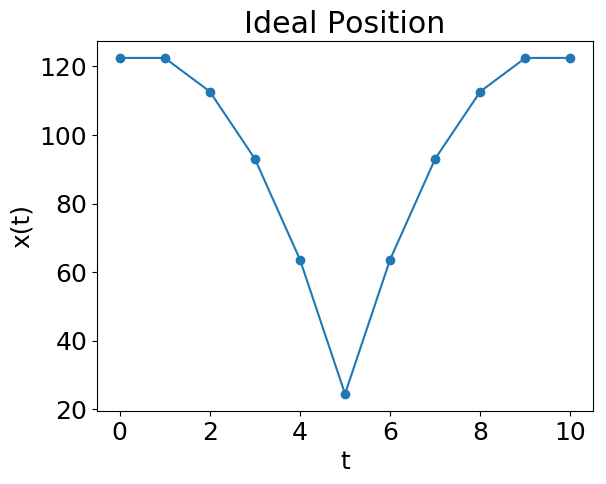
\includegraphics[width=0.48\columnwidth]{tsc-experiments/a.png}
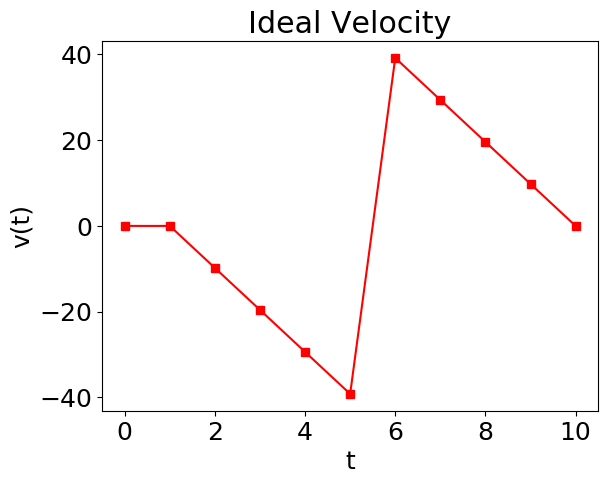
\includegraphics[width=0.48\columnwidth]{tsc-experiments/b.png}
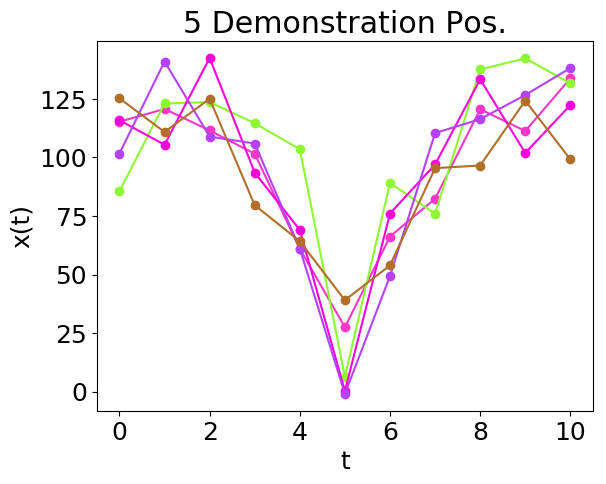
\includegraphics[width=0.48\columnwidth]{tsc-experiments/c.png}
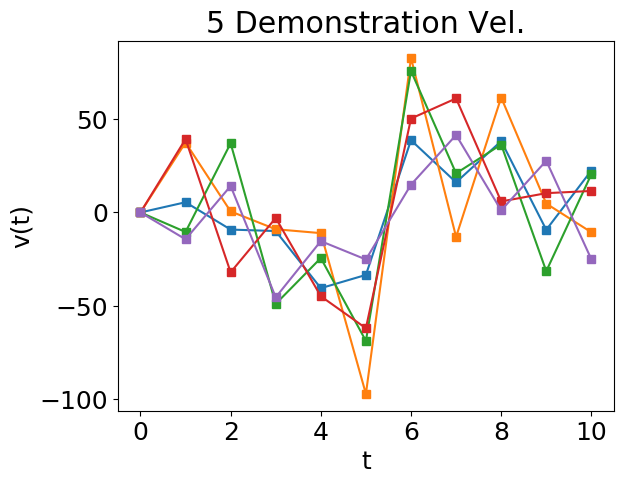
\includegraphics[width=0.48\columnwidth]{tsc-experiments/d.png}
\caption{(Above) The position and velocity of the bouncing ball without noise. (Below) 5 trajectories of the ball with different realizations of the noise. \label{ball-diagram}}
% \vspace{-1em}
\end{figure}

\begin{figure}%[t]
\centering
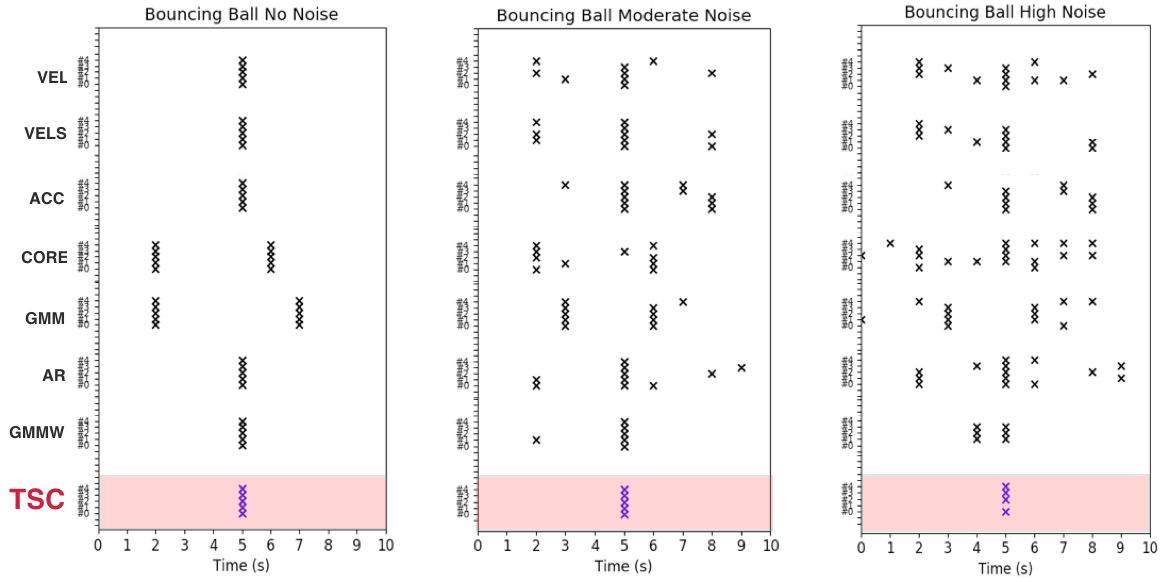
\includegraphics[width=\columnwidth]{tsc-experiments/ball-results.png}
\caption{Plots the identified transitions with each segmentation algorithm with and without noise. While all techniques are precise when there is no noise, \tsc is the most robust in the presence of noise. \label{ball-results}}
% \vspace{-1em}
\end{figure}


\textbf{Bouncing Ball: }
We first revisit the example in the introduction of the bouncing ball, which can be modeled as the following 1D double-integrator system:
\[ \ddot{x} = \unitfrac[-9.8]{\metre}{\second^2} \]
This system is observed with additive Gaussian white noise with std. 10 (Moderate Noise):
\[
y = x + N(0,10)
\]
and std. 20 (High Noise):
\[
y = x + N(0,20)
\]
The system is initialized at $x_0 = 122.5$ and bounces when $x=20$, at which point the velocity is negated.
Figure \ref{ball-diagram} illustrates the ideal trajectory and noisy realizations of these trajectories.

We apply the segmentation algorithms to the trajectories and plot the results in Figure \ref{ball-results}.
When there is no noise, all of the algorithms are equally precise, and there is no trouble corresponding segments across demonstrations.
All of the ``rate-of-change'' methods (VEL, VELS, ACC) reliably identify the point where the ball bounces.
The GMM and the Coreset methods do not segment the trajectory at the bounce point. 
On the other hand, the windowed GMM takes two consecutive positions and velocities into account during the clustering.
Similarly, the autoregressive model can accurately identify the bounce point.
With no noise, \tsc has little difference with the windowed GMM.

Differences arise when we observe the trajectory with additive Gaussian noise.
The ``rate-of-change'' methods have some spurious segmentation points due to noise. 
The GMM based methods are more robust to this noise, and they retain similar precision.
This motivates our choice of the first phase of the \tsc algorithm using a windowed GMM approach.
However, the GMM approaches still have some spurious transitions.
With these spurious points, it becomes challenging to reliably correspond trajectories across segments.
So, \tsc applies a second phase of clustering to correspond the transitions and prune the sparse clusters.
This results in accurate segmentation even in the presence of noise.

As the noise increases, \tsc is still able to find accurate segments.
In the high noise case, the bounce point is still identified in 4 out of 5 trajectories.
It is important to note that we do not claim that one segmentation algorithm is more accurate than another, or that \tsc more accurately reflects ``real'' segments.
These results only suggest that \tsc is more precise than alternatives; that is, given the assumptions in \tsc it consistently recovers segments according to those assumptions.
The next experiments will study the recall characteristics.

\begin{figure}%[t]
\centering
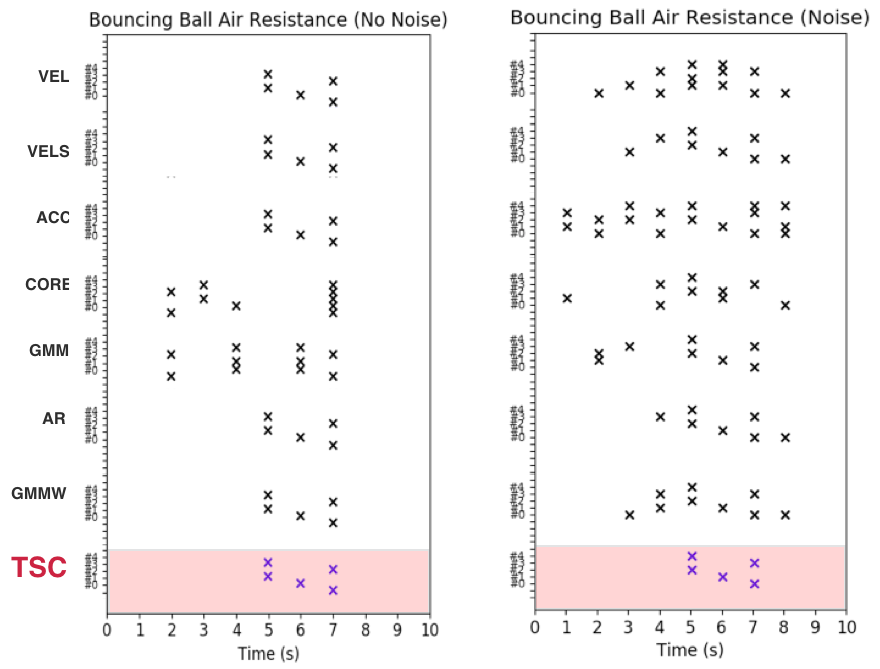
\includegraphics[width=\columnwidth]{tsc-experiments/ball-results2.png}
\caption{Plots the identified transitions with each segmentation algorithm with and without noise. In this example, temporal variation is added by incorporating a random ``air resistance'' factor.
\tsc is consistent even in the presence of this temporal variation. \label{ball-results2}}
% \vspace{-1em}
\end{figure}

\textbf{Bouncing Ball with Air Resistance: }
In the first set of experiments, we illustrate \tsc's robustness to variance in the state-space.
Next, we illustrate how \tsc can still correspond segments with temporal variation.
Consider the dynamics of the bouncing ball with an term to account for air resistance:
\[ \ddot{x} = \unitfrac[-9.8]{\metre}{\second^2} + K_v \dot{x} \]
We draw the air-resistance constant $K_v$ uniformly from $K_v \sim U[1,5]$.
The consequence is that that the ball will bounce at different times in different trajectories.

Figure \ref{ball-results2} illustrates the results.
In the 5 trajectories, the ball bounces between time-step 5 and 7.
With no noise VEL, VELS, ACC, GMMW, and \tsc can identify the bounce point.
Then, the system is observed with additive Gaussian white noise with std. 10:
\[
y = x + N(0,10)
\]
We find that \tsc recovers a consistent set of segments even with the temporal variation.

\begin{figure}%[t]
\centering
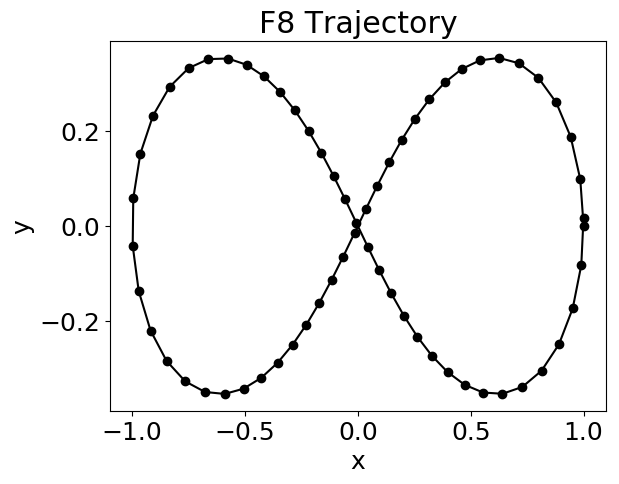
\includegraphics[width=0.48\columnwidth]{tsc-experiments/a1.png}
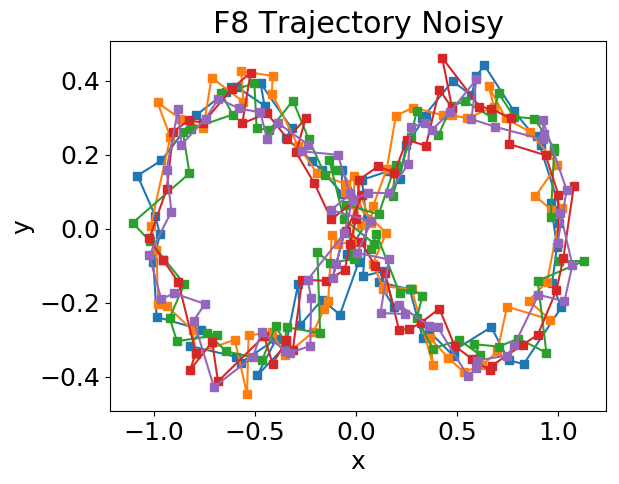
\includegraphics[width=0.48\columnwidth]{tsc-experiments/b1.png}
\caption{A ``figure 8'' trajectory in the plane, and 5 noisy demonstrations. The trajectory starts at the far right and progresses until it returns to the same spot. \label{f8-diagram}}
% \vspace{-1em}
\end{figure}

\begin{figure}%[t]
\centering
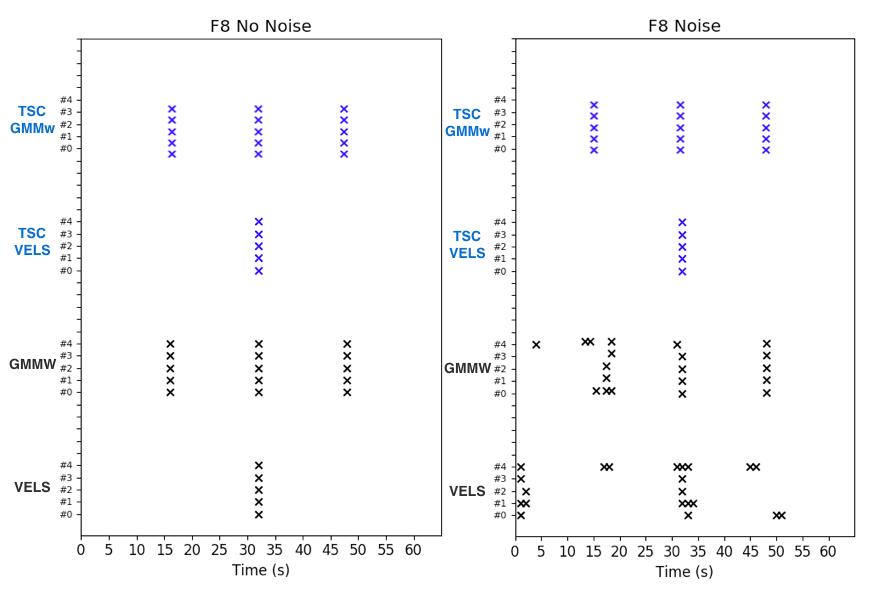
\includegraphics[width=\columnwidth]{tsc-experiments/hybrid_approach.png}
\caption{Plots the identified transitions with each segmentation algorithm with and without noise. Velocity based segmentation finds one transition point where there is a change in direction. A windowed GMM where the number of clusters is set by a DP finds three transition points. \tsc can improve the precision of both techniques.  \label{f8-results}}
% \vspace{-1em}
\end{figure}


\textbf{Hybrid Approaches: } In the previous experiments, we presented \tsc using a windowed GMM approach to identify transitions. Next, we consider \tsc with alternative transition identification functions.
Consider a ``Figure 8'' trajectory defined parametrically as:
\[
x = \textbf{cos}(t)
\]
\[
y = 0.5\textbf{sin}(2t)
\]
The trajectory is visualized in Figure \ref{f8-diagram}. The trajectory starts at the far right and progresses until it returns to the same spot. Velocity based segmentation finds one transition point where there is a change in direction (far left of the trajectory) (Figure \ref{f8-results}). 
A windowed GMM where the number of clusters is set by a DP finds three transition points. 
These three points correspond to the far left point as well as the crossing point in the figure 8 (happens twice).
These are two different segmentation criteria, and both are reasonable with respect to their respective assumptions.

Next, this parametric trajectory is observed with additive Gaussian noise of std. 0.1 (Figure \ref{f8-diagram}).
We see that both the GMM approach and the velocity approach have several spurious transitions (Figure \ref{f8-results}).
\tsc can improve the precision of both techniques by adding a layer of clustering.

\subsubsection{Rotations}
Handling orientations is a challenging problem due to the topology of $SO(3)$~\cite{ude2014orientation}. 
As an example of what can go wrong consider a 2D square rotating in the plane.
We construct a 1x1 meter 2D square and track a point on the corner of the 2D square.
The 2D square rotates clockwise in $\frac{\pi}{10}$ radian/s for 
10 time-steps, then switches, and rotates the other direction at the same angular speed.
The state of the system is the $(x,y)$ position of the corner.
We add .1 meter standard deviation Gaussian observation noise to the observed trajectories.

\begin{figure}%[t]
\centering
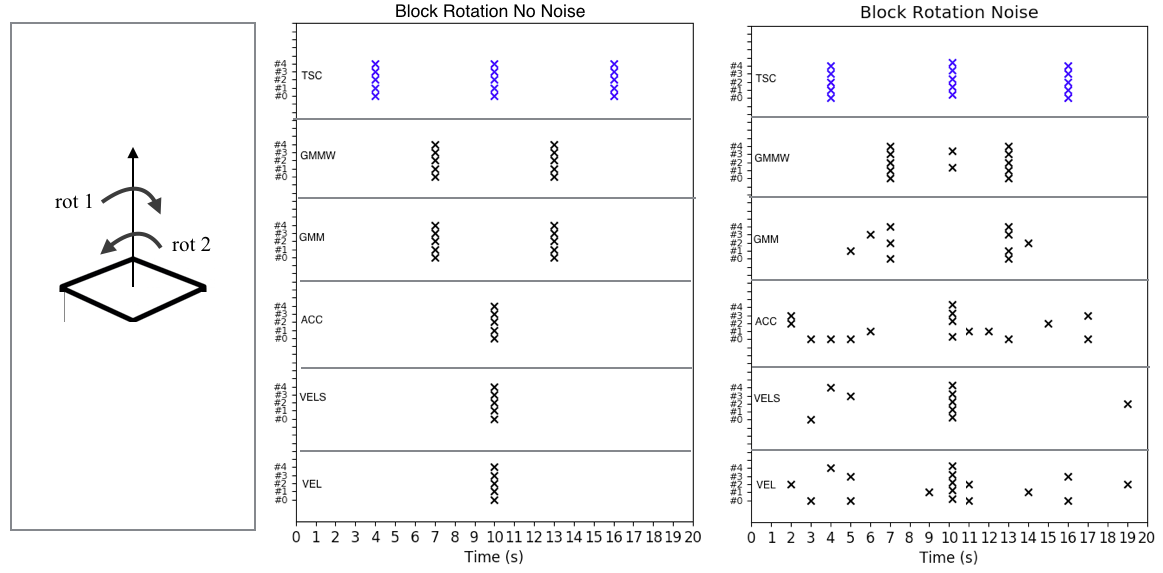
\includegraphics[width=\columnwidth]{tsc-experiments/block-results2.png}
\caption{Plots the identified transitions with each segmentation algorithm with and without noise. While all techniques are precise when there is no noise, \tsc is the most robust in the presence of noise but finds additional segments. \label{block-results}}
% \vspace{-1em}
\end{figure}


We apply the segmentation algorithms to 5 trajectories and plot the results in Figure \ref{block-results}.
As before, with no noise, all of the techniques are equally precise.
In this example, there is a difference between how the different techniques segment the trajectories.
The rate-of-change methods segment the trajectory at the point when the block changes rotation direction.
The GMM and the windowed GMM approaches cuts the trajectory into 3 even segments--missing the direction change.
\tsc cuts the trajectory into 4 segments including the direction change.
\tsc differs from the windowed GMM because it sets the number of clusters using the Dirichlet Process prior.
With noise, the rate-of-change techniques have a number of spurious segments.
The GMM-based approaches are more robust and \tsc improves the windowed GMM even further by clustering the detected transitions.
However, if the initial transitions were found in angular space, then \tsc would have found one segment.
In this sense, the definition of the state-space changes the segments found.
We hope to explore these issues in more detail in future work.


\begin{figure*}%[t]
\centering
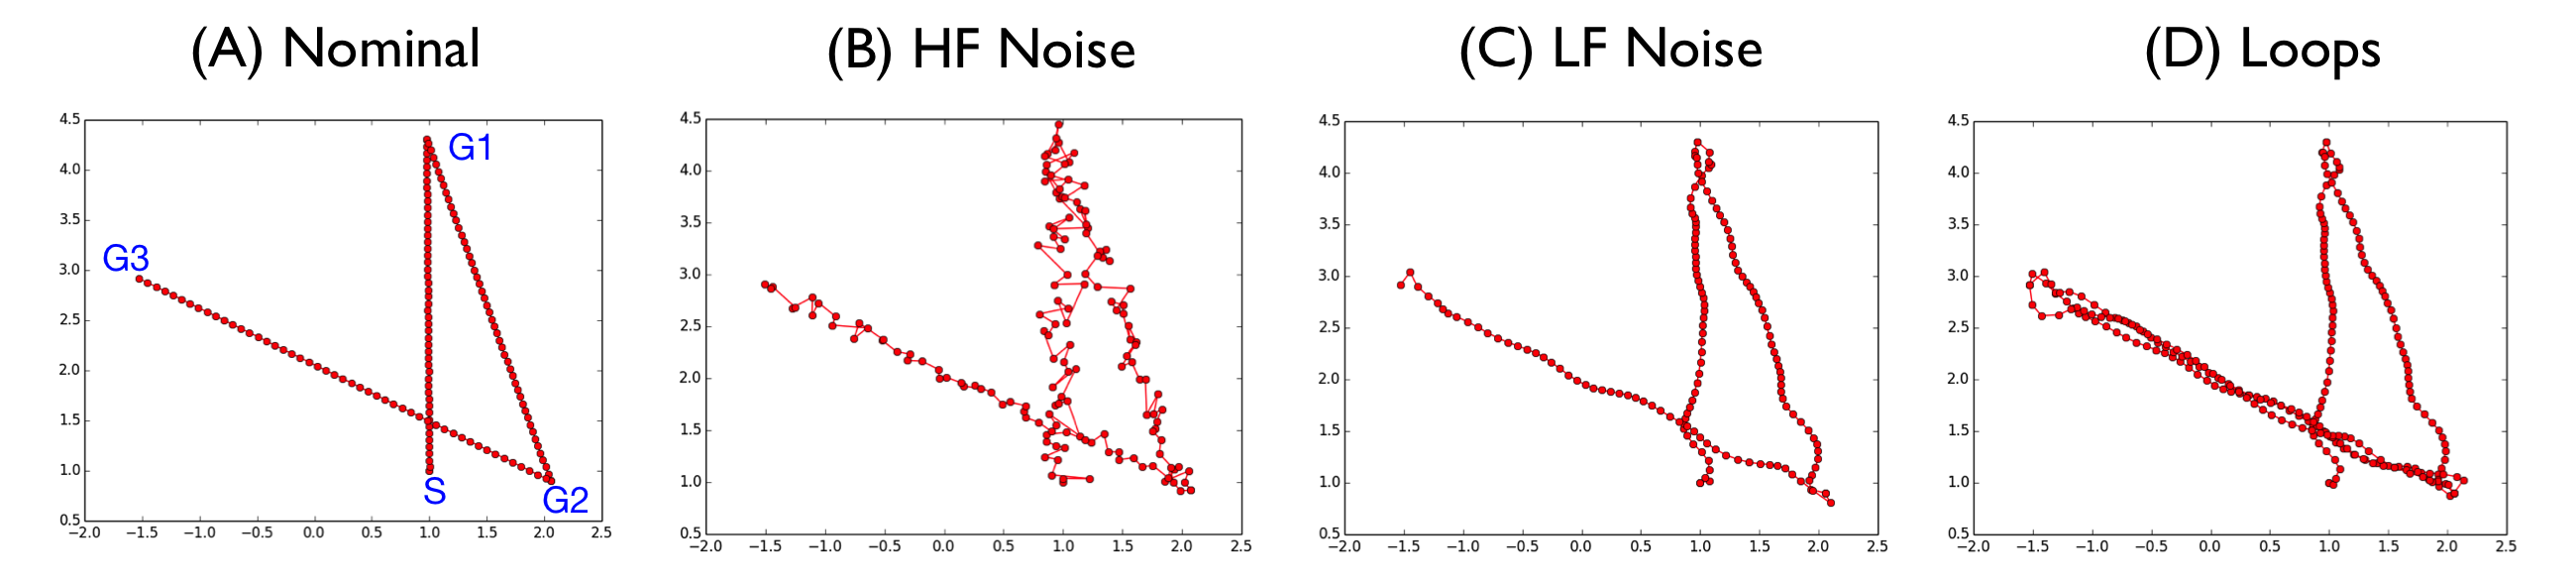
\includegraphics[width=\textwidth]{tsc-experiments/tsc_segmentation_benchmark.png}
\caption{One of 20 instances with random goal points $G1$, $G2$, $G3$. (a) Observations from a simulated demonstration with three regimes, (b) Observations corrupted with Gaussian white sensor noise, (c) Observations corrupted with low frequency process noise, and (d) Observations corrupted with an inserted loop. See Figure~\ref{exp3} for evaluation on loops. \label{simulated}}
% \vspace{-1em}
\end{figure*}

\begin{figure*}%[t]
\centering
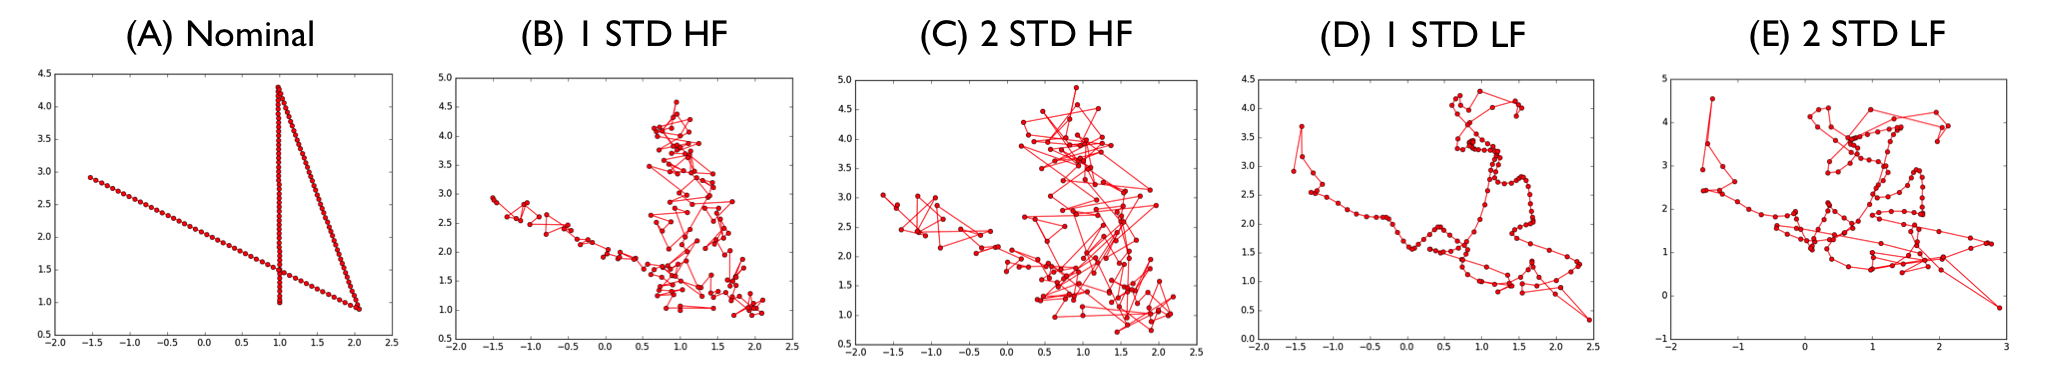
\includegraphics[width=\textwidth]{tsc-experiments/noise_illustration.png}
\caption{(a) Nominal trajectory, (b) 1 std. of high frequency observation noise, (c) 2 std. of high frequency observation noise,  (d) 1 std. of low frequency process noise, and (e) 2 std. of low frequency process noise. \label{simulated-noise}}
% \vspace{-1em}
\end{figure*}

\subsubsection{Recall in Synthetic Examples}
Comparing different segmentation models can be challenging due to differing segmentation criteria. However, we identified some algorithms that identify locally linear or near linear segments.
We developed a synthetic dataset generator to generate piecewise linear segments and compared the algorithms on the generated dataset.
Note, we do not intend this to be a comprehensive evaluation of the accuracy of the different techniques, but more a characterization of the approaches on a locally linear example to study the key tradeoffs.

We model the trajectory of a point robot with two-dimensional position state $(x,y)$ between $k$ goal points $\{g_1,...,g_k\}$. 
We apply position control to guide the robot to the targets and without disturbance, this motion is linear (Figure \ref{simulated}a).
We add various types of disturbances (and in varying amounts) including Gaussian observation noise, low-frequency process noise, and repetitive loops (Figure \ref{simulated}b-d).
We report noise values in terms of standard deviations. Figure \ref{simulated-noise} illustrates the relative magnitudes.
A demonstration $d_i$ is a sample from the following system.

\vspace{0.5em}
\noindent\textbf{Task: } Every segmentation algorithm will be evaluated in its ability to identify the $k-1$ segments (i.e., the paths between the goal points).
Furthermore, we evaluate algorithms on random instances of this task.
In the beginning, we select $3$ random goal points.
From a fixed initial position, we control the simulated point robot to the goal points with position control. 
Without any disturbance, this follows a linear motion.
For a given noise setting, we sample demonstrations from this system and apply/evaluate each algorithm.
We present results aggregated over 20 such random instances.
This is important since many of the segmentation algorithms proposed in literature have some crucial hyper-parameters, and we present results with a \emph{single} choice of parameters averaged over multiple tasks.
This way, the hyper-parameter tuning cannot overfit to any given instance of the problem and has to be valid for the entire class of tasks.
We believe that this is important since tuning these hyper-parameters in practice (i.e., not in simulation) is challenging since there is no ground truth. 
The experimental code is available at: \url{http://berkeleyautomation.github.io/tsc/}.

\vspace{0.5em}
\noindent\textbf{5 Algorithms: } We compare \tsc against alternatives where the authors explicitly find (or approximately find) locally linear segments. It is important to reiterate that different segmentation techniques optimize different objectives, and this benchmark is meant to characterize the performance on a common task. All of the techniques are based on Gaussian Distributions or Linear auto-regressive models.

\begin{figure*}
\centering
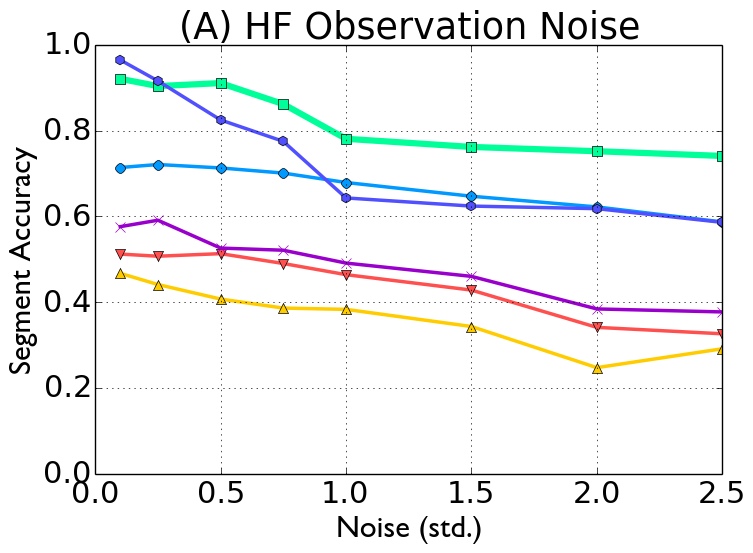
\includegraphics[width=0.33\textwidth]{tsc-experiments/exp1.png}
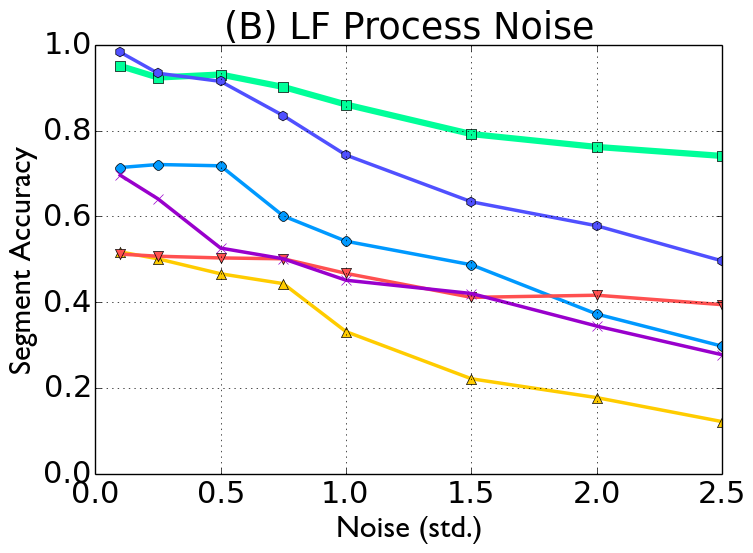
\includegraphics[width=0.33\textwidth]{tsc-experiments/exp2.png}
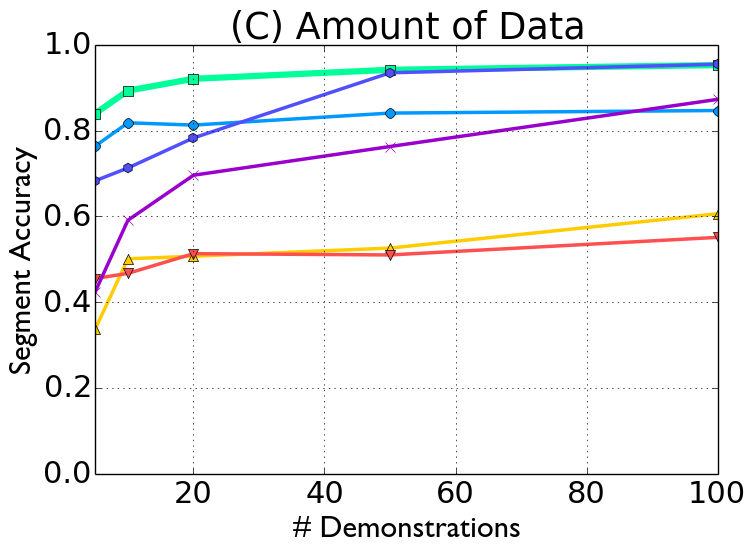
\includegraphics[width=0.33\textwidth]{tsc-experiments/exp5.png}
%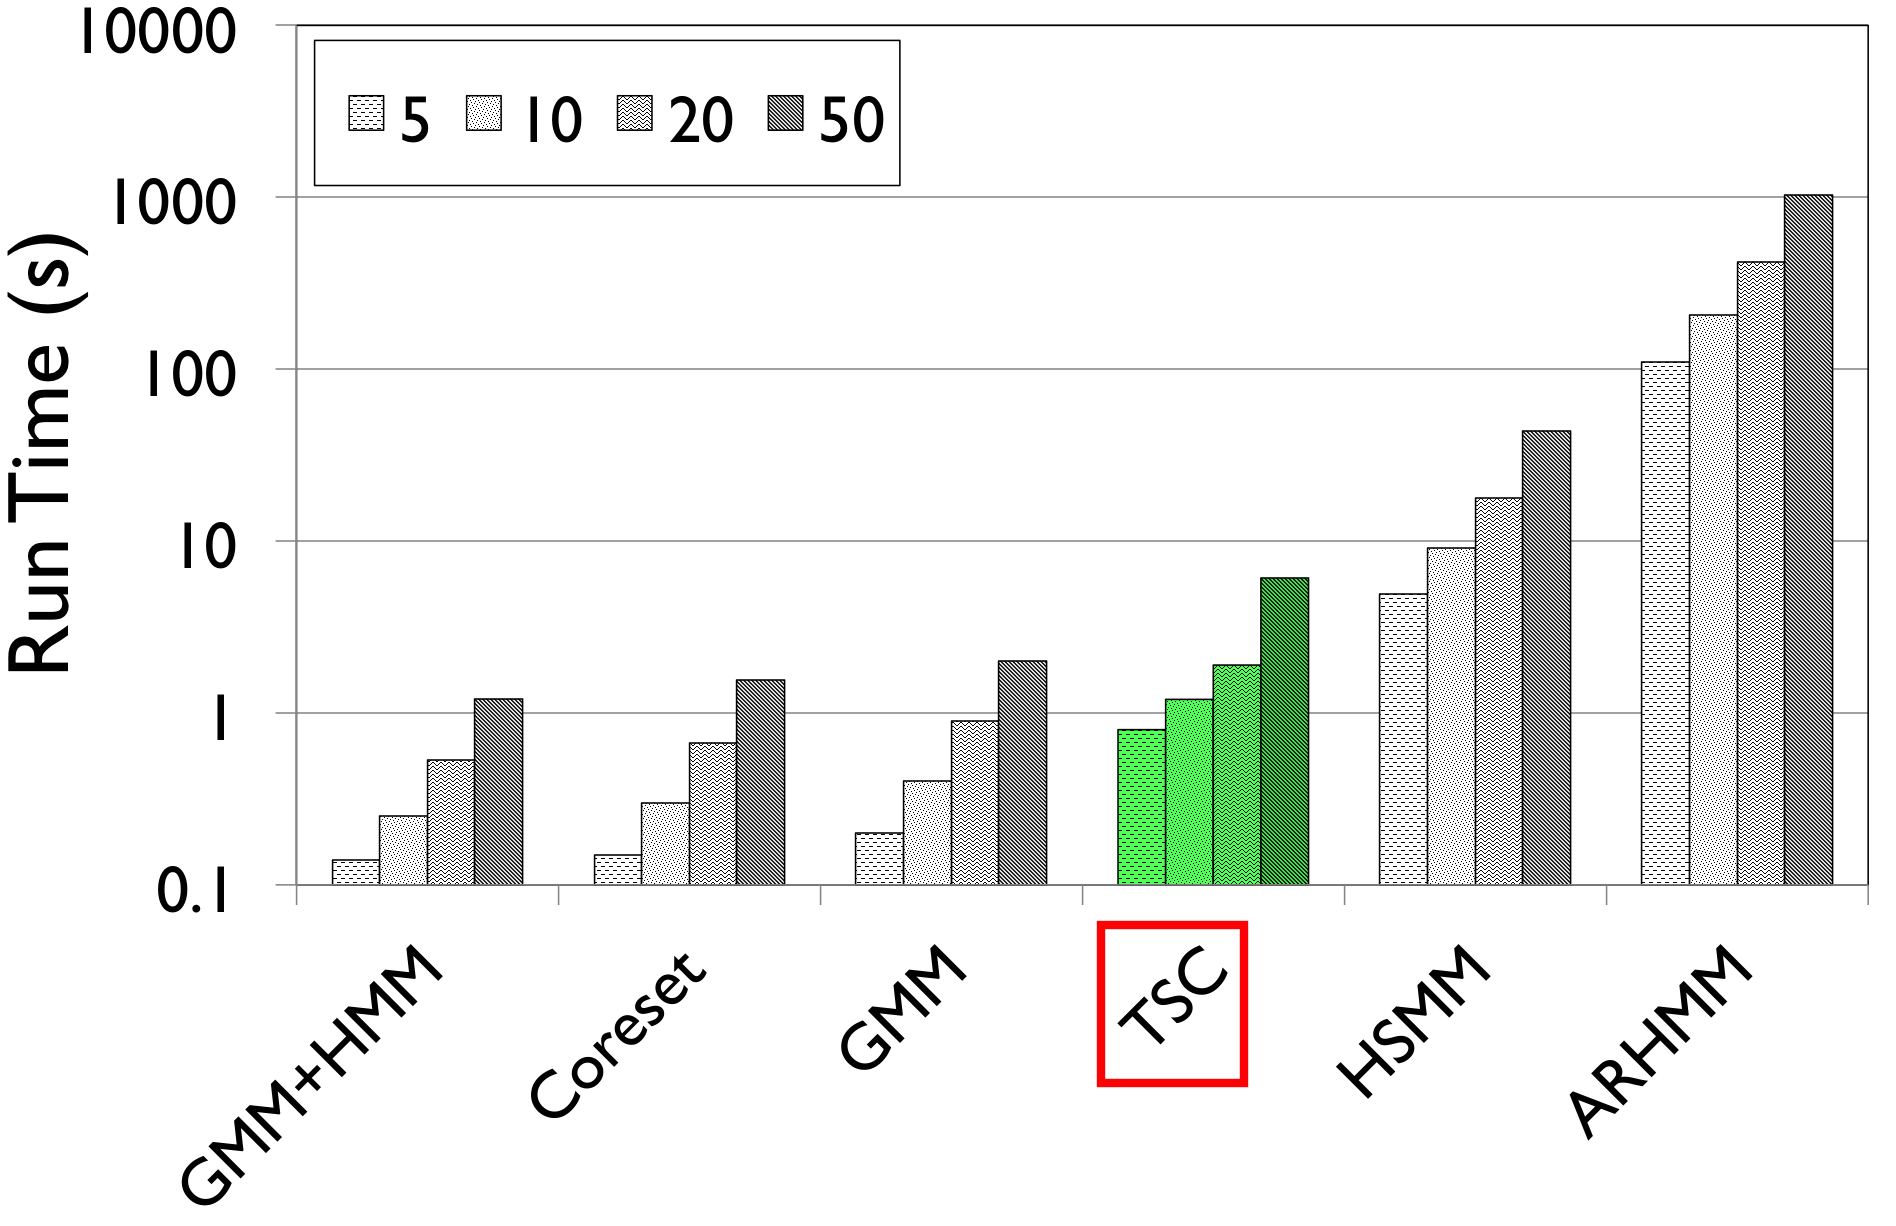
\includegraphics[width=0.24\textwidth]{tsc-experiments/bw_runtime.png}
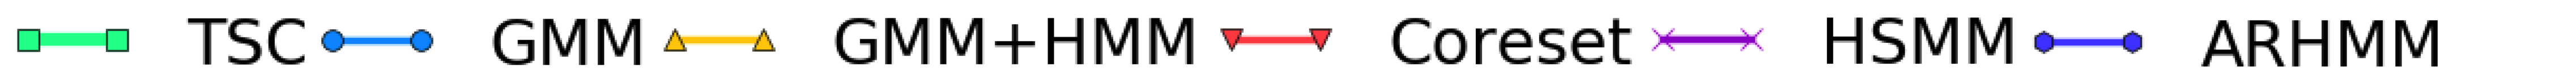
\includegraphics[width=0.8\textwidth]{tsc-experiments/big-legend.png}
\caption{Each data point represents 20 random instances of a 3-segment problem with varying levels of high-frequency noise, low-frequency noise, and demonstrations. We measure the segmentation accuracy for the compared approaches. (A) \tsc finds a more a accurate segmentation than all of the alternatives even under significant high-frequency observation noise, (B) \tsc is more robust to low-frequency process noise than the alternatives, 
% (C) \todo {\tsc performance on data with noisy loops.}
(C) the Bayesian techniques solved with MCMC (ARHMM, HSMM) are more sensitive to the number of demonstrations provided than the others.
%(D) \tsc runs over a 100x faster than the nearest alternative in terms of accuracy (ARHMM).  
\label{exp1}}
\end{figure*}

\begin{enumerate}
    \item \emph{(GMM)} (Same as previous experiment). In this experiment, we set the parameter to the optimal choice of $3$ without automatic tuning.
    \item \emph{(GMM+HMM)} A natural extension to this model is to enforce a transition structure on the regimes with a latent Markov Chain~\citep{asfour2006imitation,calinon2004stochastic,kruger2010learning, vakanski2012trajectory}. 
    We use the same state vector as above, without time augmentation as this is handled by the HMM. We fit the model using the forward-backward algorithm.
    \item \emph{Coresets} (Same as previous experiment).
    \item \emph{HSMM} We evaluated a Gaussian Hidden Semi-Markov Model as used in \cite{tanwani2016learning}. We directly applied this model to the demonstrations with no augmentation or normalization of features. This was implemented with the package \textsf{pyhsmm}. We directly applied this model to the demonstrations with no augmentation as in the GMM approaches. We ran our MCMC sampler for 10000 iterations, discarding the first 2500 as burn-in and thinning the chain by 15. 
    \item \emph{AR-HMM} We evaluated a Bayesian Autoregressive HMM model as used in \cite{niekum2012learning}. This was implemented with the packages \textsf{pybasicbayes} and \textsf{pyhsmm-ar}. The autoregressive order was $10$ and we ran our MCMC sampler for 10000 iterations, discarding the first 2500 as burn-in and thinning the chain by 15. 
\end{enumerate}

\vspace{0.5em}
\noindent\textbf{Evaluation Metric: } There is considerable debate on metrics to evaluate the accuracy of unsupervised segmentation and activity recognition techniques, e.g. frame accuracy ~\citep{wu2015watch}, hamming distance~\citep{fox2009sharing}. Typically, these metrics have two steps: (1) segments to ground truth correspondence, and (2) then measuring the similarity between corresponded segments. We have made this feature extensible and evaluated some different accuracy metrics (Jaccard Similarity, Frame Accuracy, Segment Accuracy, Intersection over Union). We found that the following procedure led to the most insightful results--differentiating the different techniques.

In the first phase, we match segments in our predicted sequence to those in the ground truth. We do this with a procedure identical to the one proposed in~\cite{wu2015watch}. We define a bi-partite graph of predicted segments to ground truth segments, and add weighted edges where weights represent the overlap between a predicted segment and a ground-truth segment (i.e., the recall over time-steps). Each predicted segment is matched to its highest weighted ground truth segment. Each predicted segment is assigned to exactly one ground-truth segment, while a ground-truth segment may have none, one, or more corresponding predictions.

After establishing the correspondence between predictions and ground truth, we consider a true positive (a ground-truth segment is correctly identified) if the overlap (intersection-over-union) between the ground-truth segment and its corresponding predicted segments is more than a default threshold 60\%.  Then, we compute \textsf{Segment Accuracy} as the ratio of the ground-truth segments that are correctly detected. In~\cite{wu2015watch}, the authors use a 40\% threshold but apply the metric to real data. Since this is a synthetic example, we increase this threshold to 60\%, which we empirically found accounted for boundary effects especially in the Bayesian approaches (i.e., repeated transitions around segment endpoints).

% In the second phase, we count the number of prediction-ground truth pairs where the intersection-over-union of time-steps is greater than 0.6 (a corresponded segment is predicted with at least 60\% accuracy). 
% We call this metric \textsf{Segment Accuracy} as in~\cite{wu2015watch}.
% The reported metric is an average over all predicted segments. 

%\subsubsection{Overview}

\begin{figure}[t]
\centering
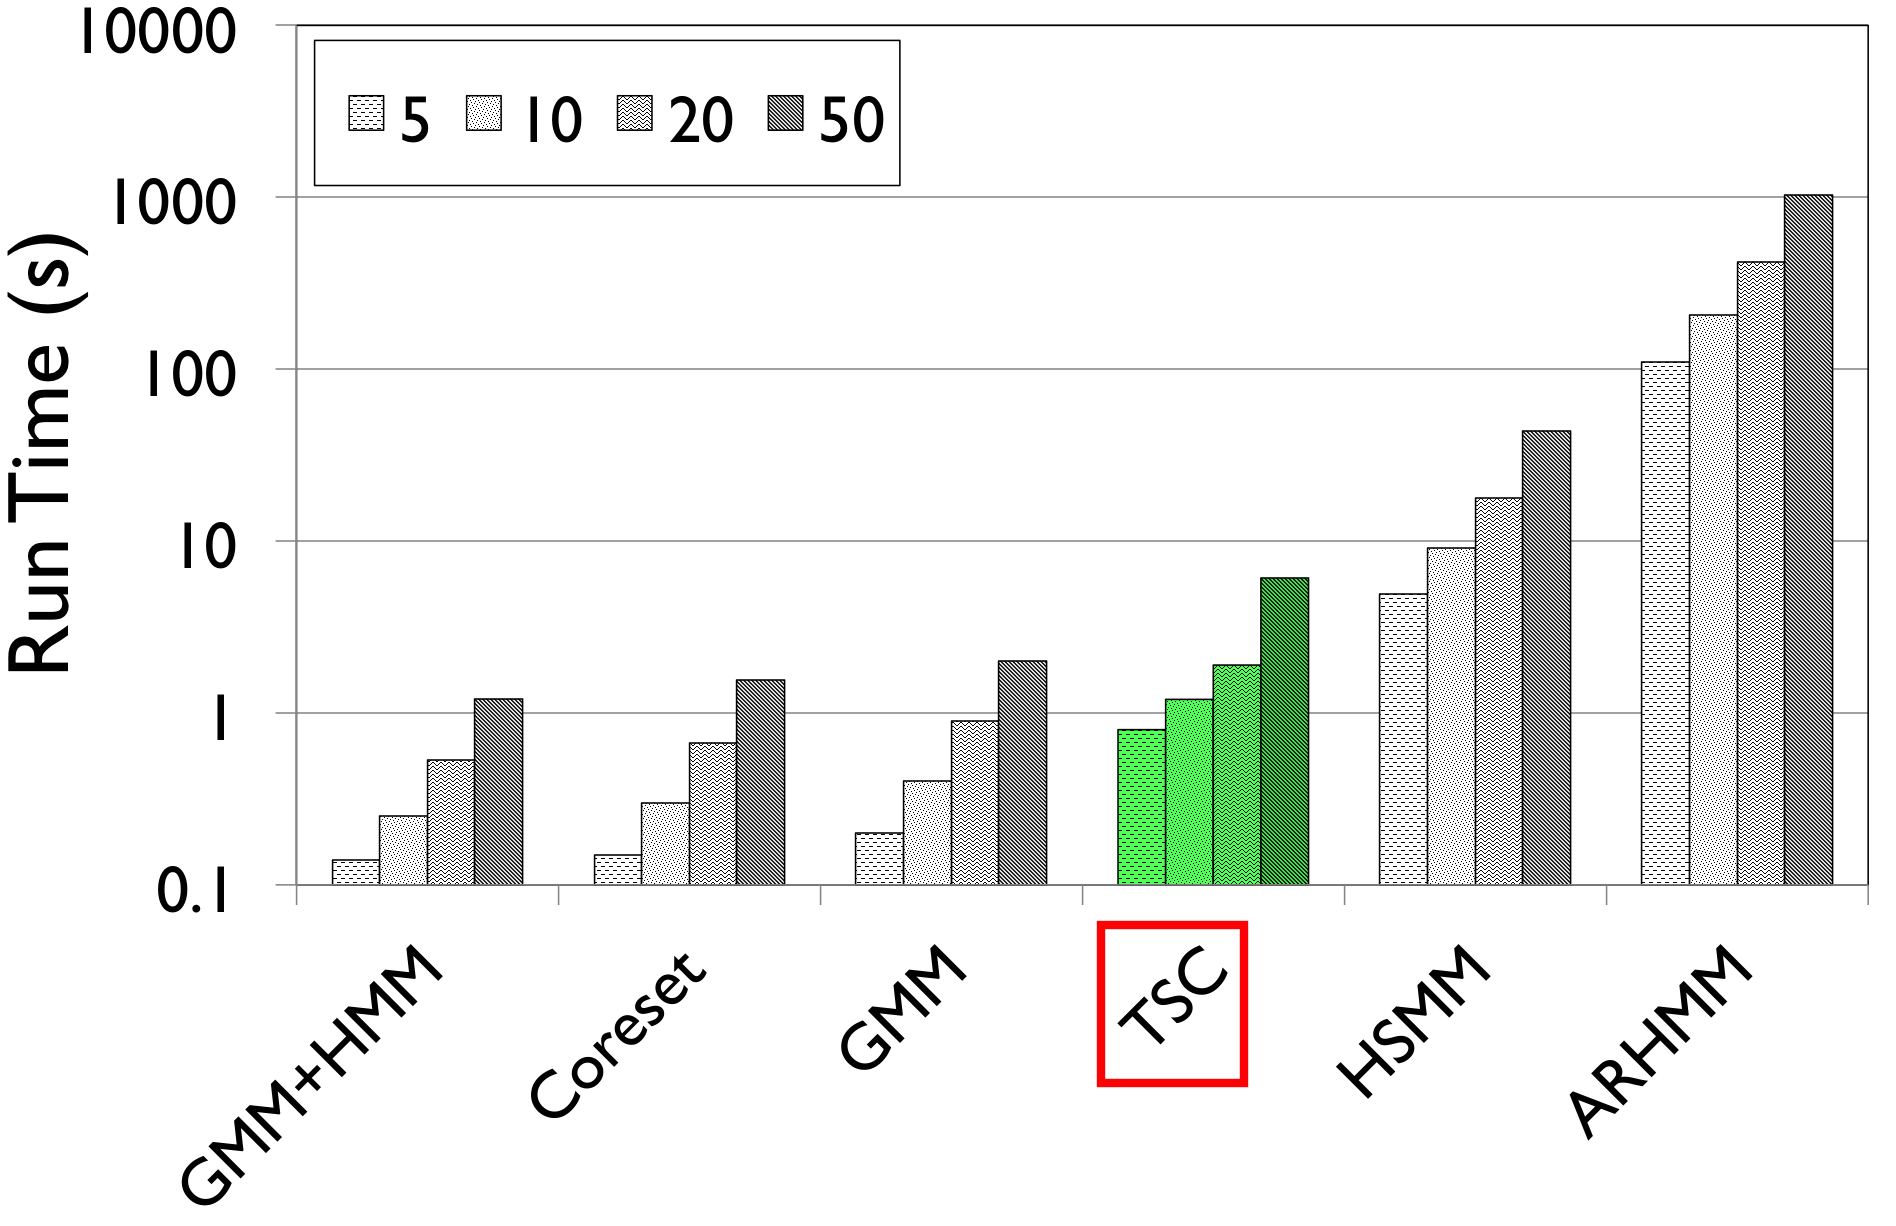
\includegraphics[width=0.8\columnwidth]{tsc-experiments/bw_runtime.png}
\caption{\tsc is about 6x slower than using Coresets or the direct GMM approach, but it is over 100x faster than the MCMC for the ARHMM model.\label{runtime}}
\end{figure}

\subsubsection{Accuracy v.s. Noise}
In our first experiment, we measured the segment accuracy for each of the algorithms for 50 demonstrations.
We also varied the amount of process and observation noise in the system.
As Figure \ref{simulated-noise} illustrates, this is a very significant amount of noise in the data, and successful techniques must exploit the structure in multiple demonstrations.
Figure \ref{exp1}a illustrates the performance of each of the techniques as a function of high-frequency observation noise.
Results suggest that \tsc is more robust to noise than the alternatives (nearly 20\% more accurate for 2.5 std of noise).
The Bayesian ARHMM approach is nearly identical to \tsc when the noise is low but quickly loses accuracy as more noise is added.
We attribute this robustness to the \tsc's pruning step which ensures that only transition state clusters with sufficient coverage across all demonstrations are kept.
These results are even more pronounced for low-frequency process noise (Figure \ref{exp1}b). \tsc is 49\% more accurate than all competitors for 2.5 std of noise added.
We find that the Bayesian approaches are particularly susceptible to such noise.
Furthermore, Figure \ref{exp1}c shows \tsc requires no more data than the alternatives to achieve such robustness.
Another point to note is that \tsc is solved much more efficiently than ARHMM or HSMM which require expensive MCMC samples.
While parameter inference on these models can be solved more efficiently (but approximately) with Mean-Field Stochastic Variational Inference, we found that the results were not as accurate.
\tsc is about 6x slower than using Coresets or the direct GMM approach, but it is over 100x faster than the MCMC for the ARHMM model.
Figure \ref{runtime} compares the runtime of each of the algorithms as a function of the number of demonstrations.

\textbf{\tsc Hyper-Parameters: }
Next, we explored the dependence of the performance on the hyper-parameters for \tsc.
We focus on the window size and the pruning parameter.
Figure \ref{exp3}a shows how varying the window size affects the performance curves.
Larger window sizes can reject more low-frequency process noise.
However, larger windows are also less efficient when the noise is low.
Similarly, Figure \ref{exp3}b shows how increasing the pruning parameter affects the robustness to high-frequency observation noise.
However, a larger pruning parameter is less efficient at low noise levels. 
Based on these curves, we selected $(w=3, \rho=0.3)$ in our synthetic experiments.

\begin{figure}
\centering
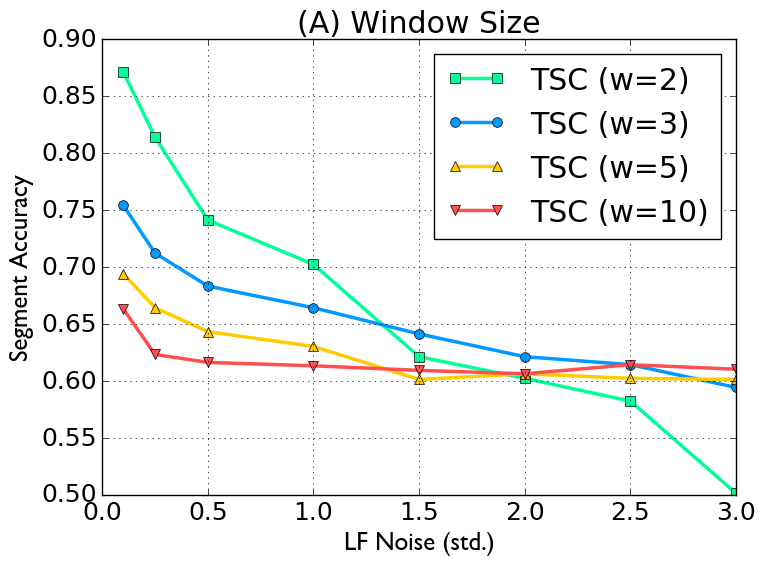
\includegraphics[width=0.48\columnwidth]{tsc-experiments/exp3.png}
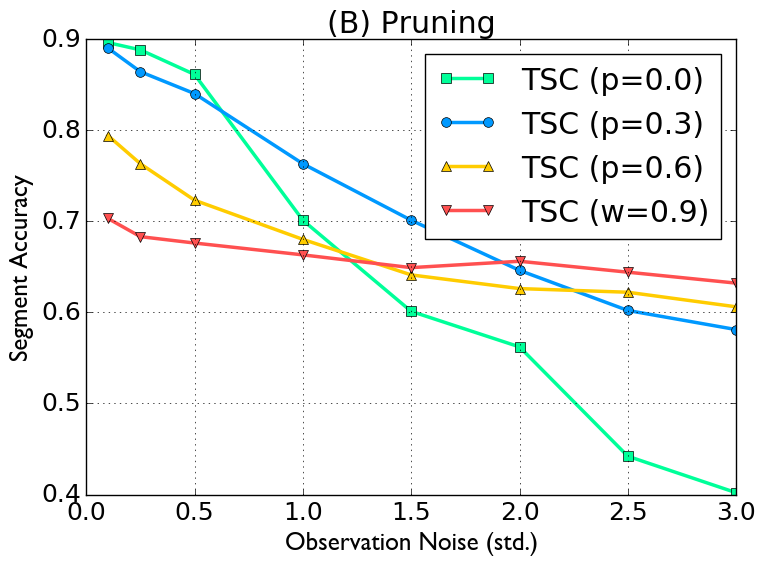
\includegraphics[width=0.48\columnwidth]{tsc-experiments/exp4.png}
\caption{(A) shows the performance curves of different choices of windows as a function of the process noise. Larger windows can reject higher amounts of process noise but are less efficient at low noise levels. (B) the performance curves of different choices of the pruning threshold. Larger pruning thresholds are more robust to high amounts of observation noise but less accurate in the low noise setting. We selected $(w=3, \rho=0.3)$ in our synthetic experiments. \label{exp3}}
\end{figure}

\textbf{Loops: }
Finally, we evaluated 4 algorithms on how well they can detect and adjust for loops.
\tsc compacts adjacent motions that are overly similar, while HMM-based approaches correspond similar looking motions.
An HMM grammar over segments is clearly more expressive than \tsc's, and we explore whether it is necessary to learn a full transition structure to compensate for loops.
We compare the accuracy of the different segmentation techniques in detecting that a loop is present (Figure \ref{exp4}).
Figure \ref{exp4}a shows that \tsc is competitive with the HMM approaches as we vary the observation noise; however, the results suggest that ARHMM provides the most accurate loop detection.
On the other hand, Figure \ref{exp4}b suggests that process noise has a very different effect.
\begin{figure}[ht]
\centering
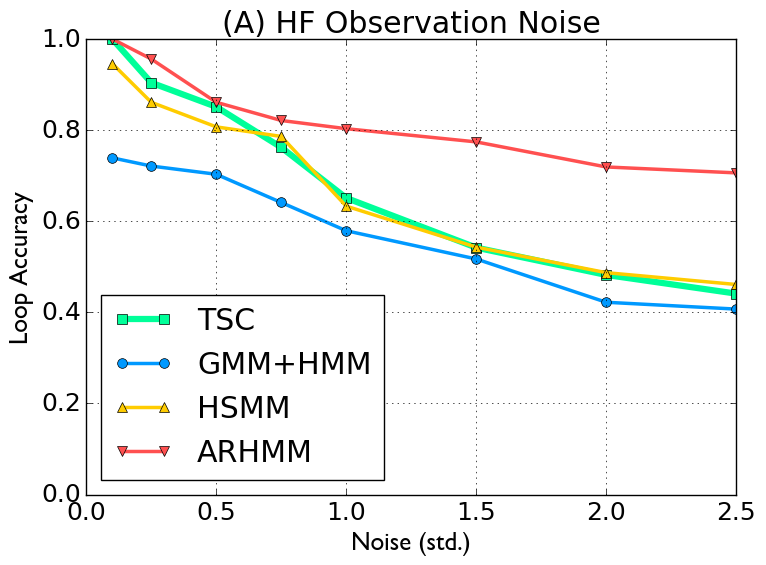
\includegraphics[width=0.48\columnwidth]{tsc-experiments/exp6.png}
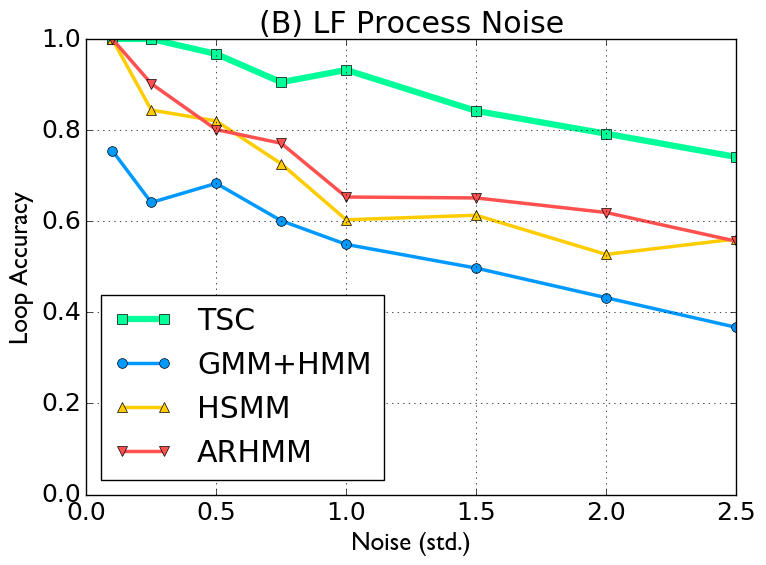
\includegraphics[width=0.48\columnwidth]{tsc-experiments/exp7.png}
\caption{(A) illustrates the accuracy of \tsc's compaction step as a function of observation noise. \tsc is competitive with the HMM-based approaches without having to model the full transition matrix. (B) \tsc is actually more robust to low-frequency process noise in the loops than the HMM-based approaches. \label{exp4}}
\end{figure}
\tsc is actually more accurate than the HMM approaches when the process noise is high--even without learning a transition structure.

\begin{figure}[ht]
\centering
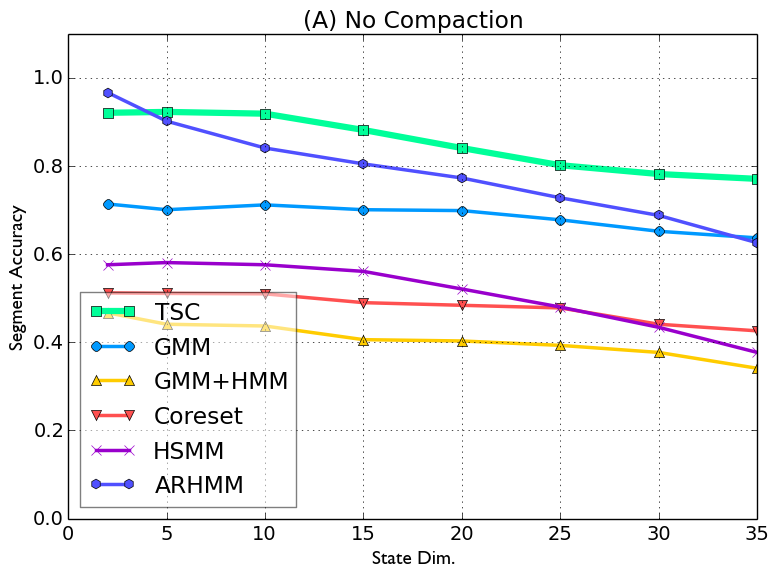
\includegraphics[width=0.48\columnwidth]{tsc-experiments/exp11.png}
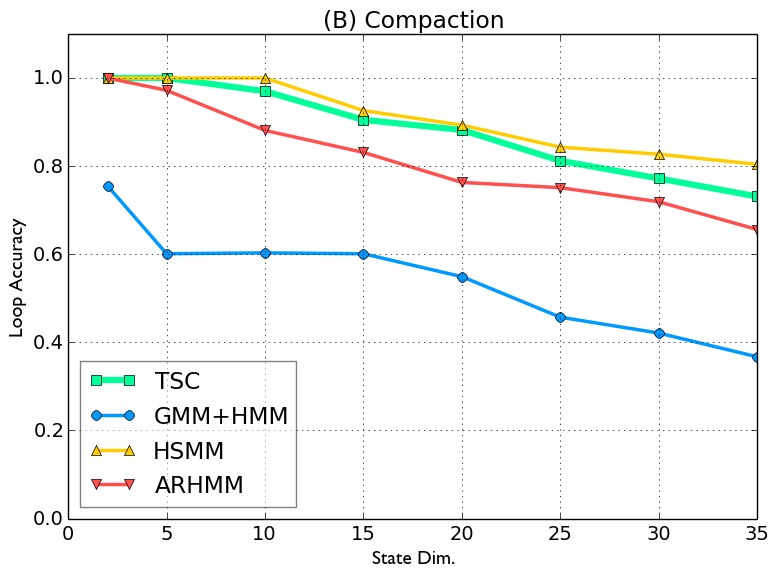
\includegraphics[width=0.48\columnwidth]{tsc-experiments/exp12.png}
\caption{We investigate how the accuracy of \tsc scales with the dimensionality of the state-space. In (A) we consider the problem with no loops or compaction, and in  (B) we measure the accuracy of the compaction step as a function of dimensionality. \label{exps}}
\end{figure}

\textbf{Scaling with Dimensionality: }
We investigate how the accuracy of \tsc scales with the dimensionality of the state-space.
As in the previous experiments, we measured the segment accuracy for each of the algorithms for 50 demonstrations.
This time we generated the line segments in increasingly higher dimensional spaces (from 2-D to 35-D).
The noise added to the trajectories has a std of 0.1.
Figure \ref{exps}a plots the segment accuracy as a function of the dimensionality of the state-space.
While the accuracy of \tsc does decreases as the dimensionality increases it is more robust than some of the alternatives: ARHMM and HSMM.
One possible explanation is that both of those techniques rely on Gibbs Sampling for inference, which is a little more sensitive to dimensionality than the expectation-maximization inference procedure used in GMM and GMM+HMM.
Figure \ref{exps}b shows one aspect of \tsc that is more sensitive to the dimensionality.
The loop compaction step requires a dynamic time-warping and then a comparison to fuse repeated segments together.
This step is not as robust in higher dimensional state-spaces.
This is possibly due to the use of the $L_2$ distance metric to compare partial trajectories to compact.
\tsc runs in $4$ seconds on the 2-D case, $16$ seconds on the 10-D case, and in $59$ seconds on the 35-D case. 



\begin{figure*}[t]
\centering
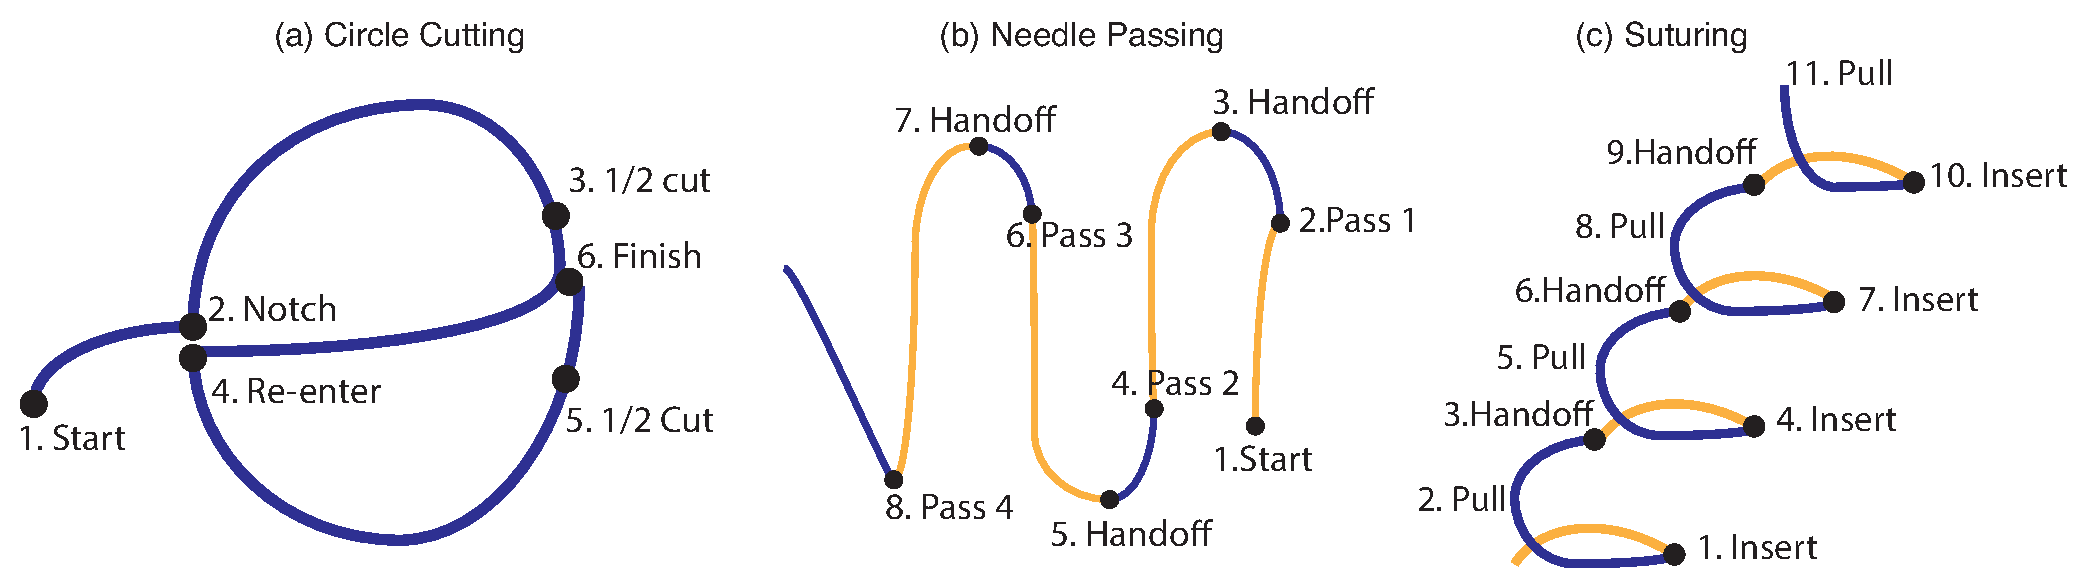
\includegraphics[width=0.7\textwidth]{tsc-experiments/conceptual_plots}
 \caption{Hand annotations of the three tasks: (a) circle cutting, (b) needle passing, and (c) suturing. Right arm actions are listed in dark blue and left arm actions are listed in yellow. \label{demo}}
%  \vspace{-2em}
\end{figure*}

\subsection{Surgical Data Experiments}
We describe the three tasks used in our evaluation and the corresponding manual segmentation (Figure \ref{demo}).
This will serve as ground truth when qualitatively evaluating our segmentation on real data.
This set of experiments primarily evaluates the utility of segments learned by \tsc.
Data was collected before hand as a part of prior work.
Our hypothesis is that even though \tsc is unsupervised, it identifies segments that often align with manual annotations.
In all of our experiments, the pruning parameter $\rho$ is set to $80\%$ and the compaction heuristic $\delta$ is to 1cm.

The state-space is the 6D end-effector position.
In some experiments, we augment this state-space with the following visual features:
\begin{enumerate}
\item \emph{Grasp}. 0 if empty, 1 other wise.
\item \emph{Needle Penetration}. We use an estimate of the penetration depth based on the robot kinematics to encode this feature. 
If there is no penetration (as detected by video), the value is 0, otherwise the value of penetration is the robot's $z$ position.
\end{enumerate}
Our goal with these features was to illustrate that \tsc applies to general state-spaces as well as spatial ones, and not to address the perception problem.
These features were constructed via manual annotation, where the Grasp and Needle Penetration were identified by reviewing the videos and marking the frames at which they occurred.

\vspace{0.5em}

\noindent\textbf{Circle Cutting: }
A 5 cm diameter circle drawn on a piece of gauze.
The first step is to cut a notch into the circle.
The second step is to cut clockwise half-way around the circle.
Next, the robot transitions to the other side cutting counter clockwise.
Finally, the robot finishes the cut at the meeting point of the two cuts.
As the left arm's only action is to maintain the gauze in tension, we exclude it from the analysis. 
In Figure \ref{demo}a, we mark 6 manually identified transitions points for this task from \cite{murali2015learning}: (1) start, (2) notch, (3) finish 1st cut, (4) cross-over, (5) finish 2nd cut, and (6) connect the two cuts.
For the circle cutting task, we collected 10 demonstrations by researchers who were not surgeons but familiar with operating the da~Vinci Research Kit~(dVRK).

\vspace{0.5em}
We also perform experiments using the JIGSAWS dataset~\cite{gao2014jigsaws} consisting of surgical activity for human motion modeling. The dataset was captured using the da Vinci Surgical System from eight surgeons with different levels of skill performing five repetitions each of Needle Passing and Suturing.

\vspace{0.5em}

\noindent\textbf{Needle Passing: } We applied \tsc to 28 demonstrations of the needle passing task.
The robot passes a needle through a hoop using its right arm, then its left arm to pull the needle through the hoop. Then, the robot hands the needle off from the left arm to the right arm. This procedure is repeated four times as illustrated with a manual segmentation in Figure~\ref{demo}b.

\vspace{0.5em}

\noindent\textbf{Suturing: }Next, we explored 39 examples of a 4 throw suturing task (Figure \ref{demo}c). Using the right arm, the first step is to penetrate one of the points on right side. The next step is to force the needle through the phantom to the other side. Using the left arm, the robot pulls the needle out of the phantom and then the robot hands it off to the right arm for the next point. 

% \begin{figure}[10][!h]
%     \centering
%     % \vspace{-15pt}
%     \caption{Hand annotations of the three tasks: (a) circle cutting, (b) needle passing, and (c) suturing. Right arm actions are listed in dark blue and left arm actions are listed in yellow.}                
%     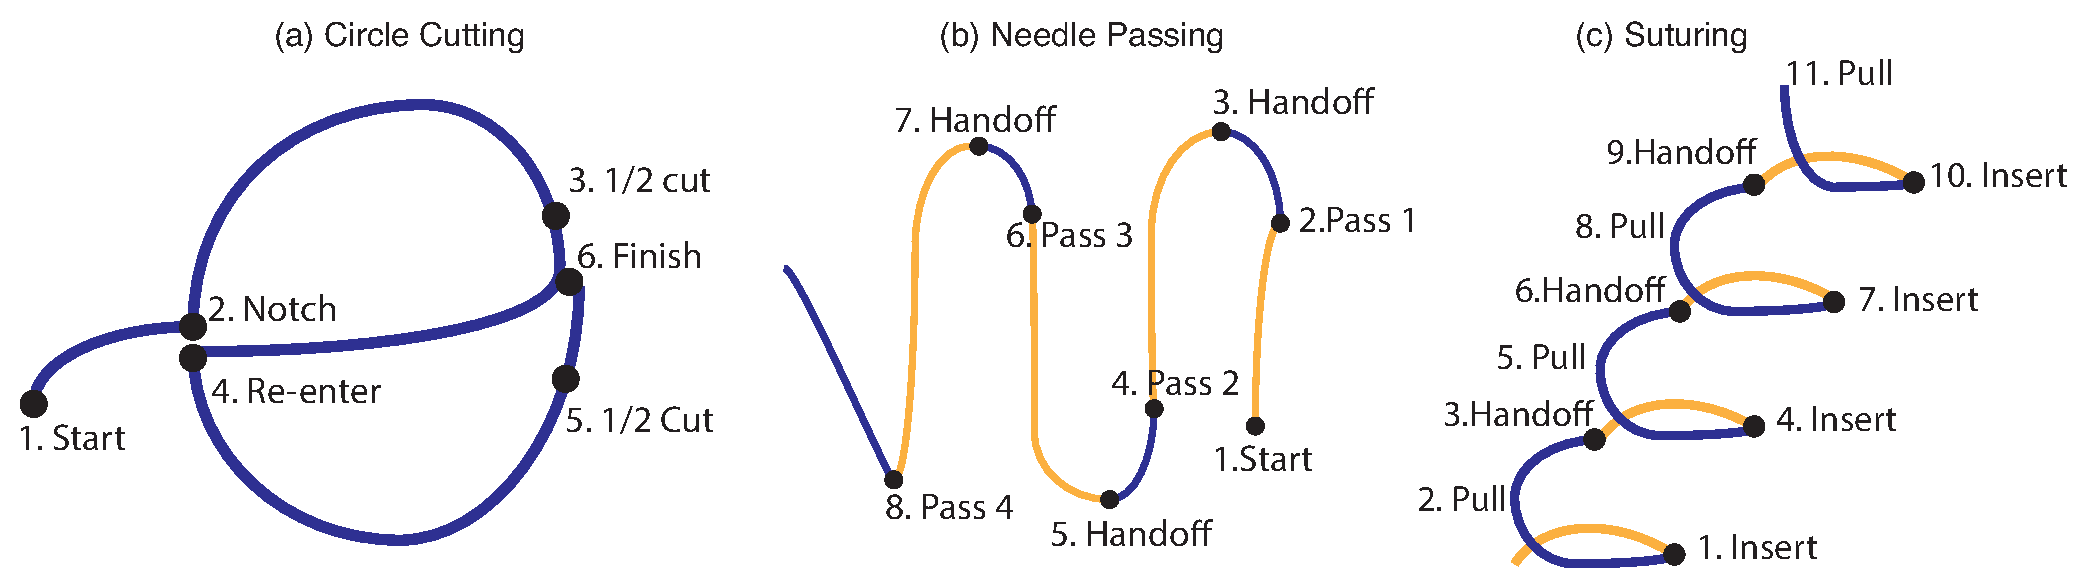
\includegraphics[width=0.6\textwidth]{tsc-experiments/conceptual_plots}
%      \label{demo}
%     \vspace{-1.5em}
% \end{figure}

\begin{figure*}[t]
\centering
    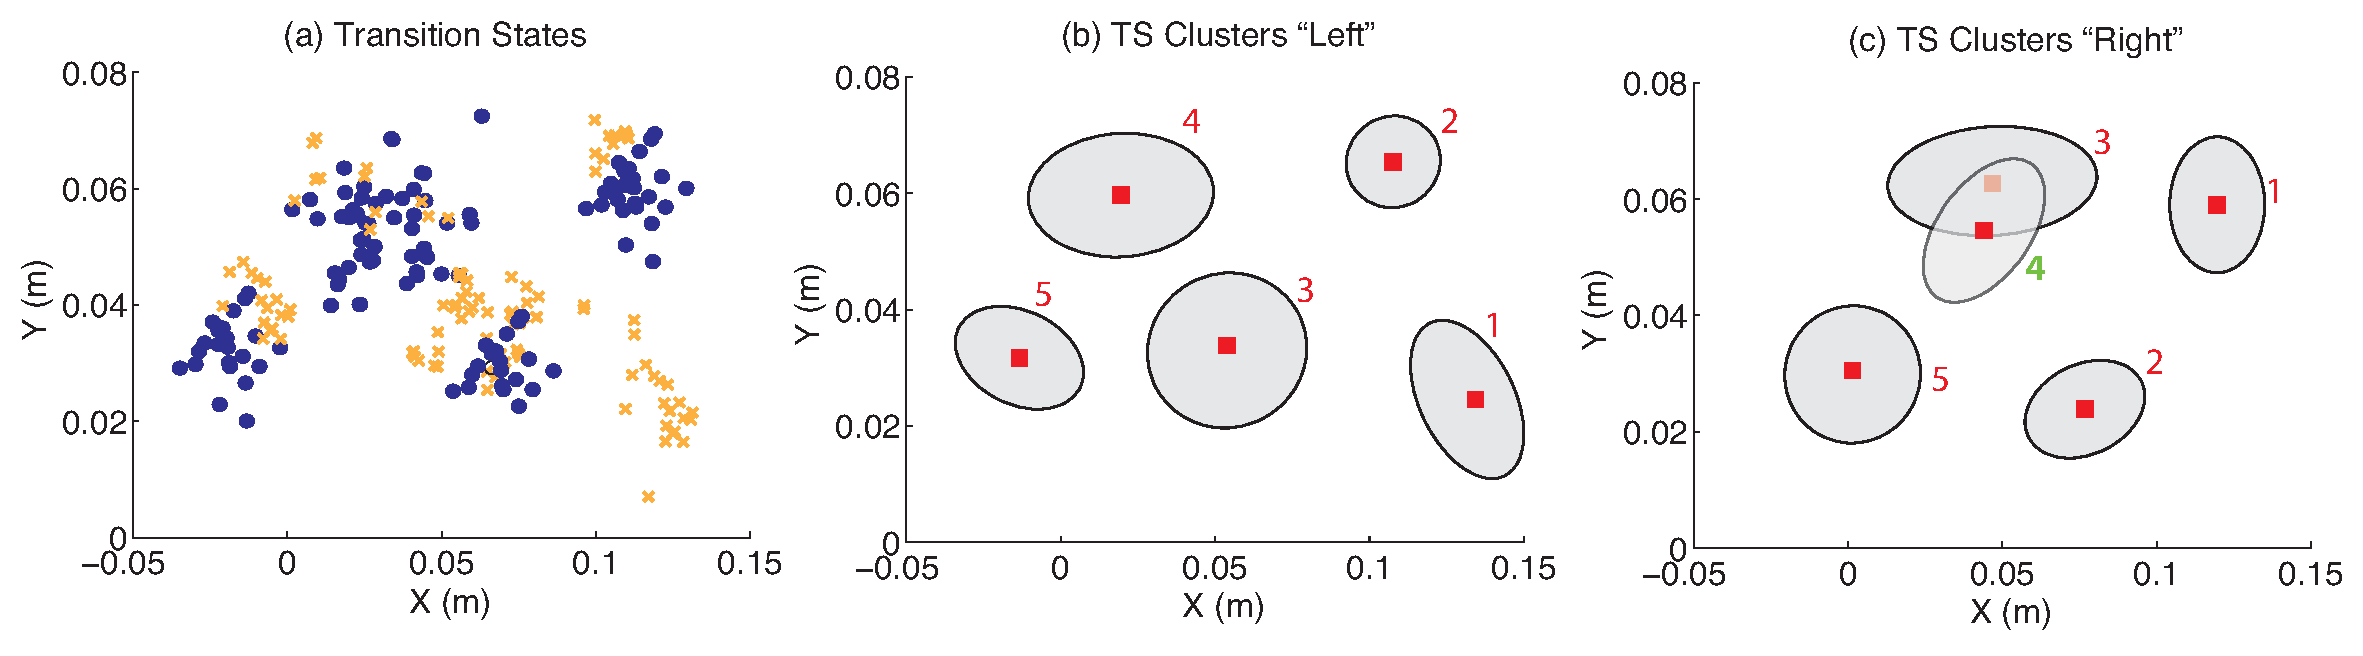
\includegraphics[width=0.8\textwidth]{tsc-experiments/new_needle_passing2.eps}
    \vspace{-0.7em}
    \caption{(a) The transition states for the task are marked in orange (left arm) and blue (right arm). (b-c) The \tsc clusters, which are clusters of the transition states, are illustrated with their 75\% confidence ellipsoid for both arms}
    \label{exp:np}
    \vspace{-0.5em}
\end{figure*}

\begin{figure*}[t]
\centering
    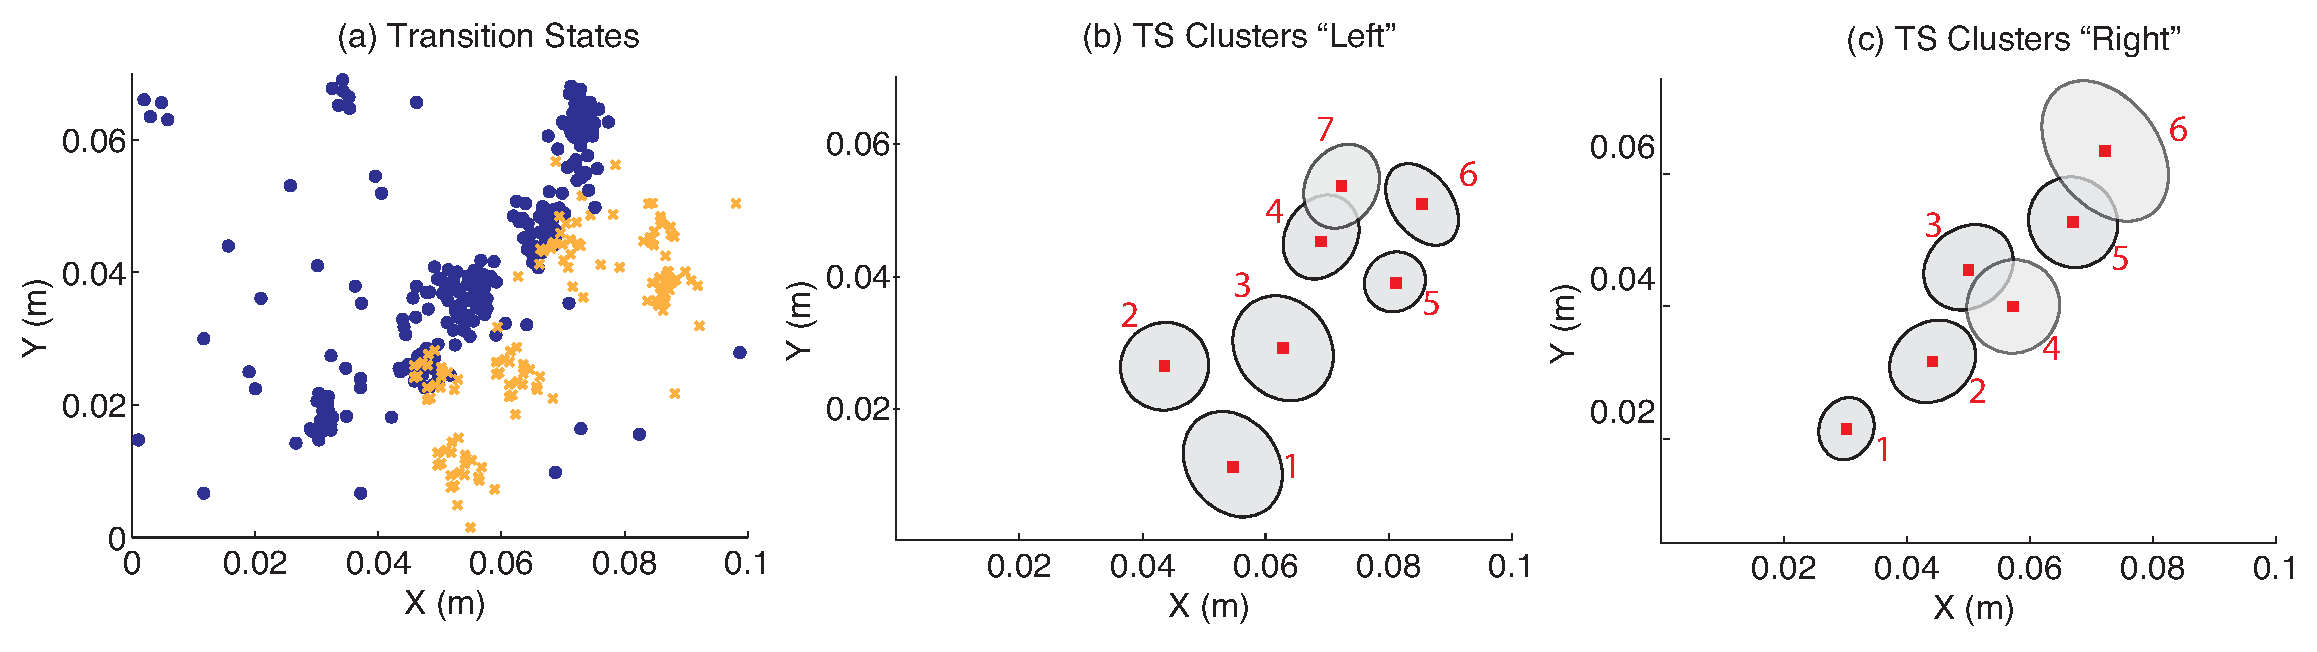
\includegraphics[width=0.8\textwidth]{tsc-experiments/new_suturing2.eps}
    \vspace{-0.7em}
    \caption{ (a) The transition states for the task are marked in orange (left arm) and blue (right arm). (b-c) The clusters, which are clusters of the transition states, are illustrated with their 75\% confidence ellipsoid for both arms}
    \label{exp:su}
    % \vspace{-0.5em}
\end{figure*}

\iffalse
\subsection{Visual Features}\label{cvh}
\tsc is compatible with visual features in addition to kinematic states.
Our goal with these features was to illustrate that \tsc applies to general state-spaces as well as spatial ones, and not to address the general perception problem.
These features were constructed via manual annotation, where the Grasp and Needle Penetration were identified by reviewing the videos and marking the frames at which they occurred.

We evaluate \tsc in this featurized state space that incorporates states derived from vision.
We illustrate the transition states in Figure~\ref{exp:cop} with and without visual features on the circle cutting task.
 At each point where the model transitions, we mark the end-effector $(x,y,z)$ location (ignoring the orientation).
 In particular, we show a region (red box) to highlight the benefits of these features.
During the cross-over phase of the task, the robot has to re-enter the notch point and adjust to cut the other half of the circle.
When only using the end-effector kinematic pose, the locations where this transition happens is unreliable as operators may approach the entry from slightly different angles.
On the other hand, the use of a gripper contact binary feature clusters the transition states around the point at which the gripper is in position and ready to begin cutting again.
In the subsequent experiments, we use the same two visual features.

\begin{figure}[t]
\centering
  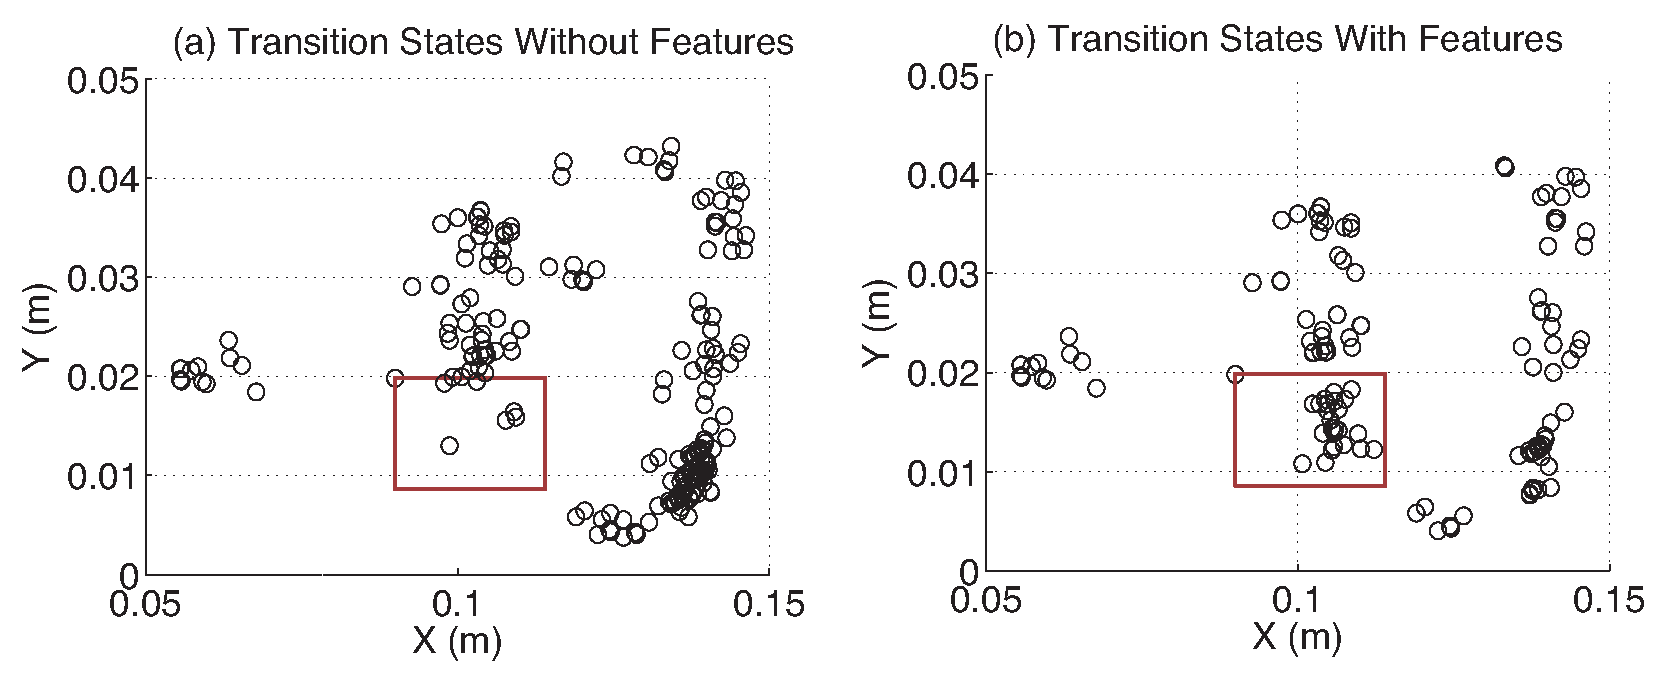
\includegraphics[width=\columnwidth]{tsc-experiments/exp1_e_state.eps}
%   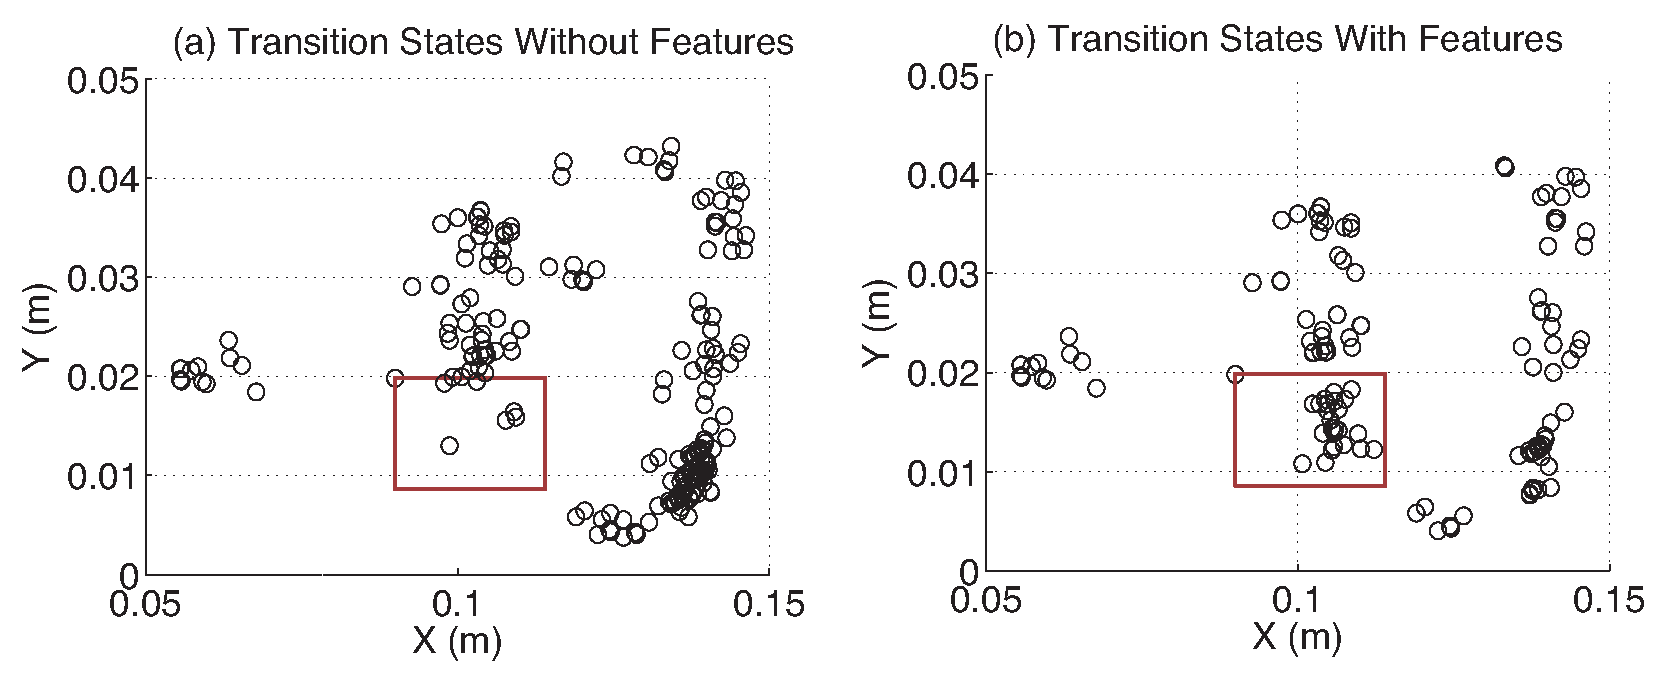
\includegraphics[width=1.4\textwidth]{tsc-experiments/exp1_e_state.eps}
 \caption{(a) We show the transition states without visual features, (b) and with visual features. Marked in the red box is a set of transitions that cannot always be detected from kinematics alone. 
 \label{exp:cop}}
\end{figure}
\fi


\subsubsection{Pruning and Compaction} \label{sec:pruningCompaction}
In Figure \ref{exp:removal}, we highlight the benefit of pruning and compaction using the Suturing task as exemplar.
First, we show the transition states without applying the compaction step to remove looping transition states (Figure \ref{exp:removal}a).
We find that there are many more transition states at the ``insert" step of the task.
Compaction removes the segments that correspond to a loop of the insertions.
Next, we show all of the clusters found by the first step of segmentation.
The centroids of these clusters are marked in Figure \ref{exp:removal}b.
Many of these clusters are small containing only a few transition states. 
This is why we created the heuristic to prune clusters that do not have transition states from at least 80\% of the demonstrations.
In all, 11 clusters are pruned by this rule.

% \begin{figure}[t]
%     \centering
%     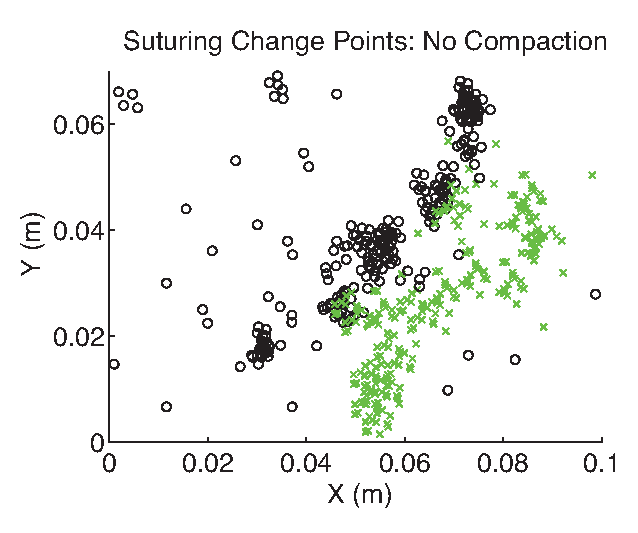
\includegraphics[width=0.35\textwidth]{tsc-experiments/suturing_milestones_no_compaction}
%     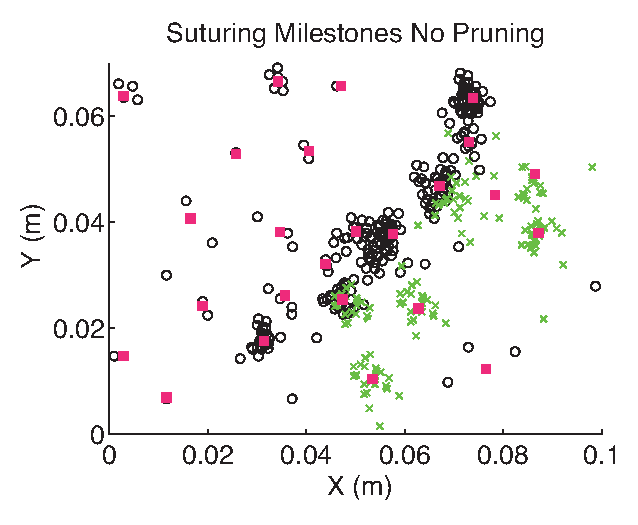
\includegraphics[width=0.35\textwidth]{tsc-experiments/suturing_milestones_no_pruning}
%     \caption{We illustrate the benefits of pruning small clusters and our retry compaction algorithm. We first show the transition states without compaction, and then show the clusters without pruning.}
%      \label{exp:removal}
% \end{figure}

\begin{figure}[t]
    \centering
    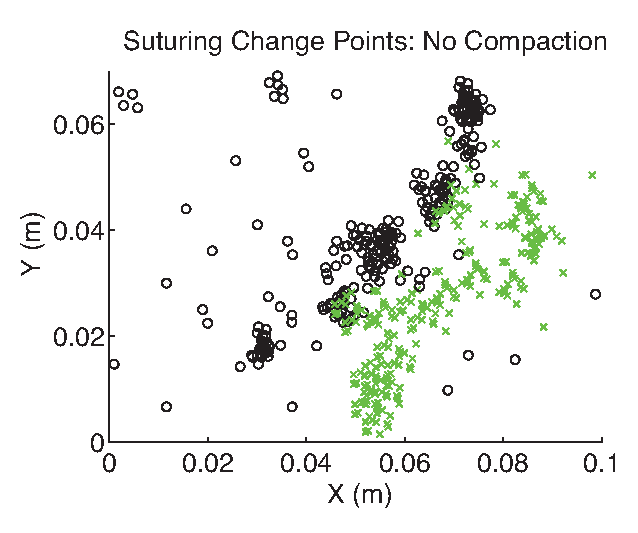
\includegraphics[width=0.45\columnwidth]{tsc-experiments/suturing_milestones_no_compaction}
    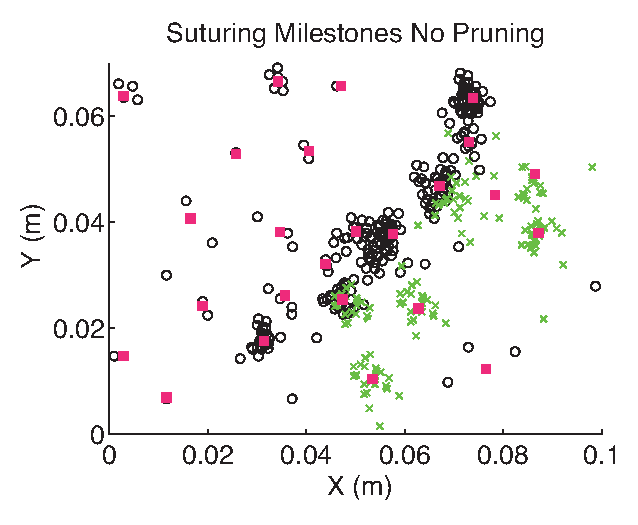
\includegraphics[width=0.45\columnwidth]{tsc-experiments/suturing_milestones_no_pruning}
    \caption{We first show the transition states without compaction (in black and green), and then show the clusters without pruning (in red). Compaction sparsifies the transition states and pruning significantly reduces the number of clusters.}
    \label{exp:removal}
\end{figure}

\begin{figure}[t]
    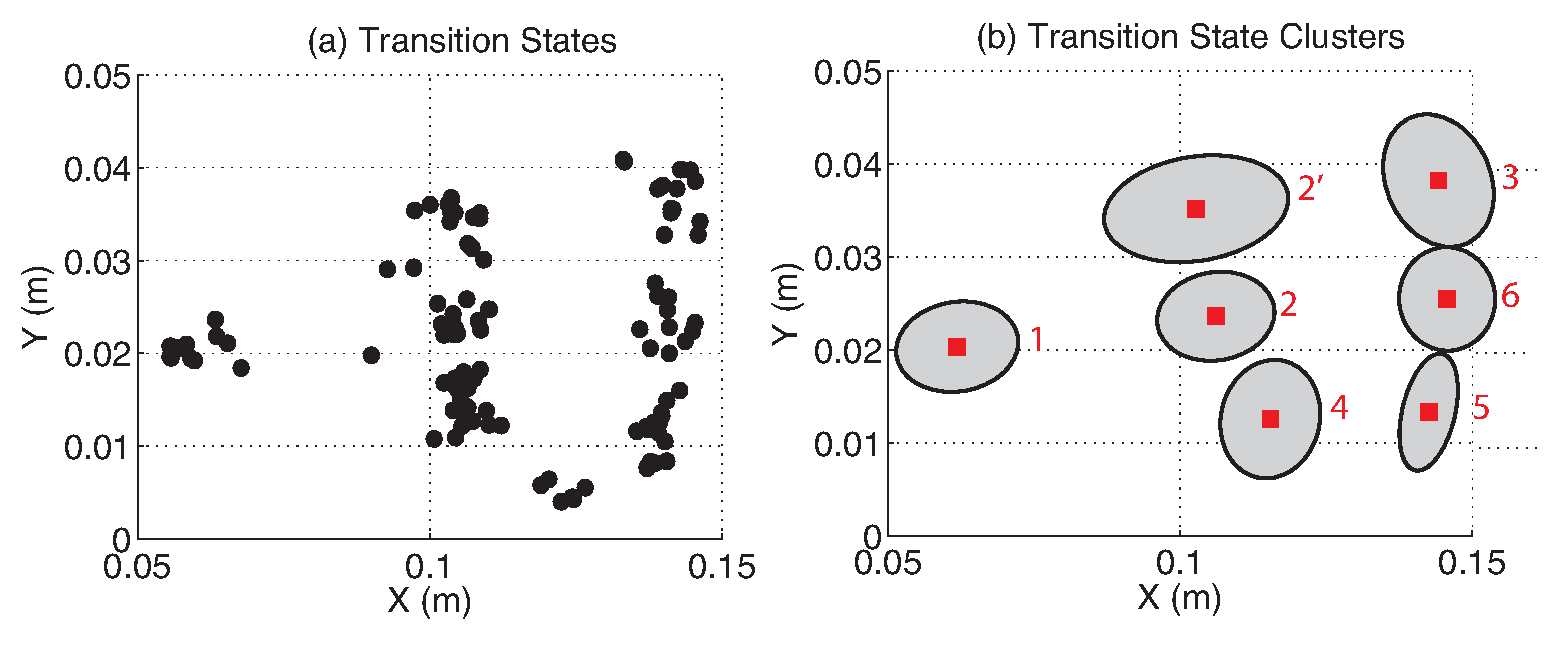
\includegraphics[width=\columnwidth]{tsc-experiments/new_circle_cutting}
    \caption{(a) The transition states for the circle cutting task are marked in black. (b) The \tsc clusters, which are clusters of the transition states, are illustrated with their 75\% confidence ellipsoid.\label{exp:circ}}
\end{figure}

\subsubsection{Results}\label{results:real}

\noindent\textbf{Circle Cutting: }
Figure\,\ref{exp:circ}a shows the transition states obtained from our algorithm. And Figure\,\ref{exp:circ}b shows the \tsc clusters learned (numbered by time interval midpoint).
The algorithm found 8 clusters, one of which was pruned using our $\rho=80\%$ threshold rule.

The remaining 7 clusters correspond well to the manually identified transition points.
It is worth noting that there is one extra cluster (marked $2'$), that does not correspond to a transition in the manual segmentation.
At $2'$, the operator finishes a notch and begins to cut.
While at a logical level notching and cutting are both penetration actions, they correspond to two different linear transition regimes due to the positioning of the end-effector.
Thus, \tsc separates them into different clusters even though the human annotators did not.
This illustrates why supervised segmentation is challenging.
Human annotators segment trajectories on boundaries that are hard to characterize mathematically, e.g., is frame 34 or frame 37 the segment boundary.
Supervisors may miss crucial motions that are useful for automation or learning.




% \vspace{0.5em}

\noindent\textbf{Needle Passing: } 
In Figure\,\ref{exp:np}a, we plot the transition states in $(x,y,z)$ end-effector space for both arms.
We find that these transition states correspond well to the logical segments of the task (Figure\,\ref{demo}b).
These demonstrations are noisier than the circle cutting demonstrations, and there are more outliers.
The subsequent clustering finds 9 clusters (2 pruned).
Next, Figures\,\ref{exp:np}b-c illustrate the \tsc clusters.
We find that again \tsc learns a small parametrization for the task structure with the clusters corresponding well to the manual segments.
However, in this case, the noise does lead to a spurious cluster (4 marked in green).
One possible explanation is that the demonstrations contain many adjustments to avoid colliding with the needle hoop and the other arm while passing the needle through leading to numerous transition states in that location.

%Our technique is not limited to x,y,z states for the robot and works with more general configurations. In Figure \ref{exp:np}b, at each of the first 5 clusters, we plot the learned mean pose. 
%This shows that the robot has to orient its end-effector horizontal to the loop during the pass through and pull and vertical during the handoff.

\vspace{0.5em}

\noindent\textbf{Suturing: }
In Figure\,\ref{exp:su}, we show the transition states and clusters for the suturing task.
As before, we mark the left arm in orange and the right arm in blue.
This task was far more challenging than the previous tasks as the demonstrations were inconsistent.
These inconsistencies were in the way the suture is pulled after insertion (some pull to the left, some to the right, etc.), leading to transition states all over the state space. 
Furthermore, there were numerous demonstrations with looping behaviors for the left arm.
In fact, the DP-GMM method gives us $23$ clusters, $11$ of which represent less than $80$\% of the demonstrations and thus are pruned (we illustrate the effect of the pruning in the next section).
In the early stages of the task, the clusters clearly correspond to the manually segmented transitions.
As the task progresses, we see that some of the later clusters do not.



\begin{table*}
\caption{This table compares transitions learned by \tsc and transitions identified by manual annotators in the JIGSAWS dataset. We found that the transitions mostly aligned. $83\%$ and $73\%$ of transition clusters for needle passing and suturing respectively contained exactly one surgeme transition when both kinematics and vision were used. Results suggest that the hierarchical clustering is more suited for mixed video and kinematic feature spaces.}
\centering
\scriptsize
\begin{tabular}{| l | c | c | c | c | c |}
\hline
 & No. of Surgeme Segments & No. of Clusters & seg-surgeme & surgeme-seg \\ 
\hline
Needle Passing TSC(Kin+Video)  & $14.4 \pm 2.57$ & 11 & 83\% & 74\% \\ \hline
Needle Passing TSC(Video) & $14.4 \pm 2.57$ & 7 & 62\% & 69\% \\ \hline
Needle Passing TSC(Kin) & $14.4 \pm 2.57$ & 16 & 87\% & 62\% \\ \hline
Needle Passing TSC(VELS) & $14.4 \pm 2.57$ & 13 & 71\% & 70\% \\ \hline
Needle Passing TSC(No-H)  & $14.4 \pm 2.57$ & 5 & 28\% & 34\% \\\hline
\hline
Suturing TSC(Kin+Video) & $15.9 \pm 3.11$ & 13 & 73\% & 66\% \\ \hline
Suturing TSC(Video) & $15.9 \pm 3.11$ & 4 & 21\% & 39\% \\ \hline
Suturing TSC(Kin) & $15.9 \pm 3.11$ & 13 & 68\% & 61\% \\ \hline
Suturing TSC(VELS) & $15.9 \pm 3.11$ & 17 & 48\% & 57\% \\ \hline
Suturing TSC(No-H) & $15.9 \pm 3.11$ & 9 & 51\% & 52\% \\ \hline
\end{tabular}
 \label{exp:surgemes}
\end{table*}


\subsubsection{Comparison to Surgemes}
%\todo{SK: Clean up the metrics}
Surgical demonstrations have an established set of primitives called surgemes, and we evaluate if segments discovered by our approach correspond to surgemes. 
In Table \ref{exp:surgemes}, we compare the number of \tsc segments for needle passing and suturing to the number of annotated surgeme segments.
We apply different variants of the \tsc algorithm and evaluate its ability to recover segments similar to surgemes.
We consider: (Kin+Video) which is the full \tsc algorithm, (Kin) which only uses kinematics, (Video) which only uses the visual annotations, (VELS) which uses the zero-crossing velocity heuristic to get the initial transitions, and (NO-H) which treats all of the variables as one big feature space and does not hierarchically cluster.
A key difference between our segmentation and number of annotated surgemes is our compaction and pruning steps.
To account for this, we first select a set of surgemes that are expressed in most demonstrations (i.e., simulating pruning), and we also apply a compaction step to the surgeme segments.
When surgemes appear consecutively, we only keep the one instance of each.
We explore two metrics: \textbf{seg-surgeme} the fraction of \tsc clusters with only one surgeme switch (averaged over all demonstrations), and \textbf{surgeme-seg} the fraction of surgeme switches that fall inside exactly one \tsc cluster.

 We found that the transitions learned by \tsc with both the kinematic and video features were the most aligned with the surgemes. 
 $83\%$ and $73\%$ of transition clusters for needle passing and suturing respectively contained exactly one surgeme transition when both were used.
 For the needle passing task, we found that the video features alone could give a reasonably accurate segmentation.
 However, this did not hold for the suturing dataset.
 The manual video features are low dimensional and tend to under-segment.
 For the suturing dataset, a combination of the visual and kinematic features was most aligned with the surgemes.
 Similarly, this scaling problem affects the variant that does not hierarchically cluster--leading to a small number of clusters--and inaccuracy.
 
 
 
 






\iffalse
\subsection{Experiment 1. Synthetic Example of 2-Segment Trajectory}\label{toy}
\todo{SK: Will remove this set of experiments for new benchmark}
In our first experiment, we segment noisy observations from a two regime linear dynamical system. 
Figure \ref{generated-data} illustrates examples from this system under the different types of corruption.
Since there is a known a ground truth of two segments, we measure the precision (average fraction of observations in each segment that are from the same regime) and recall (average fraction of observations from each regime segmented together) in recovering these two segments.
We can jointly consider precision and recall with the \emph{F1 Score} which is the harmonic mean of the two.
We compare three techniques against \tsc: K-Means (only spatial), GMM+T (using time as a feature in a GMM), GMM+HMM (using an HMM to model the grammar).
For the GMM techniques, we have to select the number of segments, and we experiment with $k=1,2,3$ (i.e., a slightly sub-optimal parameter choice compared to $k=2$).
In this example, for \tsc, we set the two user-specified parameters to $\delta=0$ (merge all repeated transitions), and $\rho=80\%$ (prune all regimes representing less than $80\%$ of the demonstrations).

First, we generate 100 noisy observations (additive zero mean Gaussian noise) from the system without loops or spurious states--effectively only measuring the DP-GMM versus the alternatives.
Figure \ref{generated-comp}a shows the F1-score as a function of the noise in the observations.
Initially, for an appropriate parameter choice $k=2$ both of the GMM-based methods perform well and at low noise levels the DP-GMM used by our work mirrors this performance.
However, if the parameter is set to be $k=3$, we see that the performance significantly degrades.
$k=1$ corresponds to a single segment which has a F1 score of 0.4 on all figures.
The DP-GMM mitigates this sensitivity to the choice of parameter by automatically setting the value.
Furthermore, as the noise increases, the $80\%$ pruning of DP-GMM mitigates the effect of outliers leading to improved accuracy. 

In Figure \ref{generated-comp}b, we look at the accuracy of each technique as a function of the number of demonstrations.
GMM+HMM has more parameters to learn and therefore requires more data.
GMM+T converges the fastest, \tsc requires slightly more data, and the GMM+HMM requires the most.
In Figure \ref{generated-comp}c, we corrupt the observations with spurious dynamical regimes. These are random transition matrices which replace one of the two dynamical regimes.
We vary the rate at which we randomly corrupt the data, and measure the performance of the different segmentation techniques as a function of this rate.
Due to the pruning, \tsc gives the most accurate segmentation. 
The Dirichlet process groups the random transitions in different clusters and the small clusters are pruned out.
On the other hand, the pure GMM techniques are less accurate since they are looking for exactly two regimes.

In Figure \ref{generated-comp}d, introduce corruption due to loops and compare the different techniques.
A loop is a step that returns to the start of the regime randomly, and we vary this random rate.
For an accurately chosen parameter $k=2$, for the GMM-HMM, it gives the most accurate segmentation.
However, when this parameter is set poorly $k=3$, the accuracy is significantly reduced.
On the other hand, using time as a GMM feature (GMM+T) does not work since it does not know how to group loops into the same regime.
\fi

\iffalse
\begin{figure*}%[t]
\centering
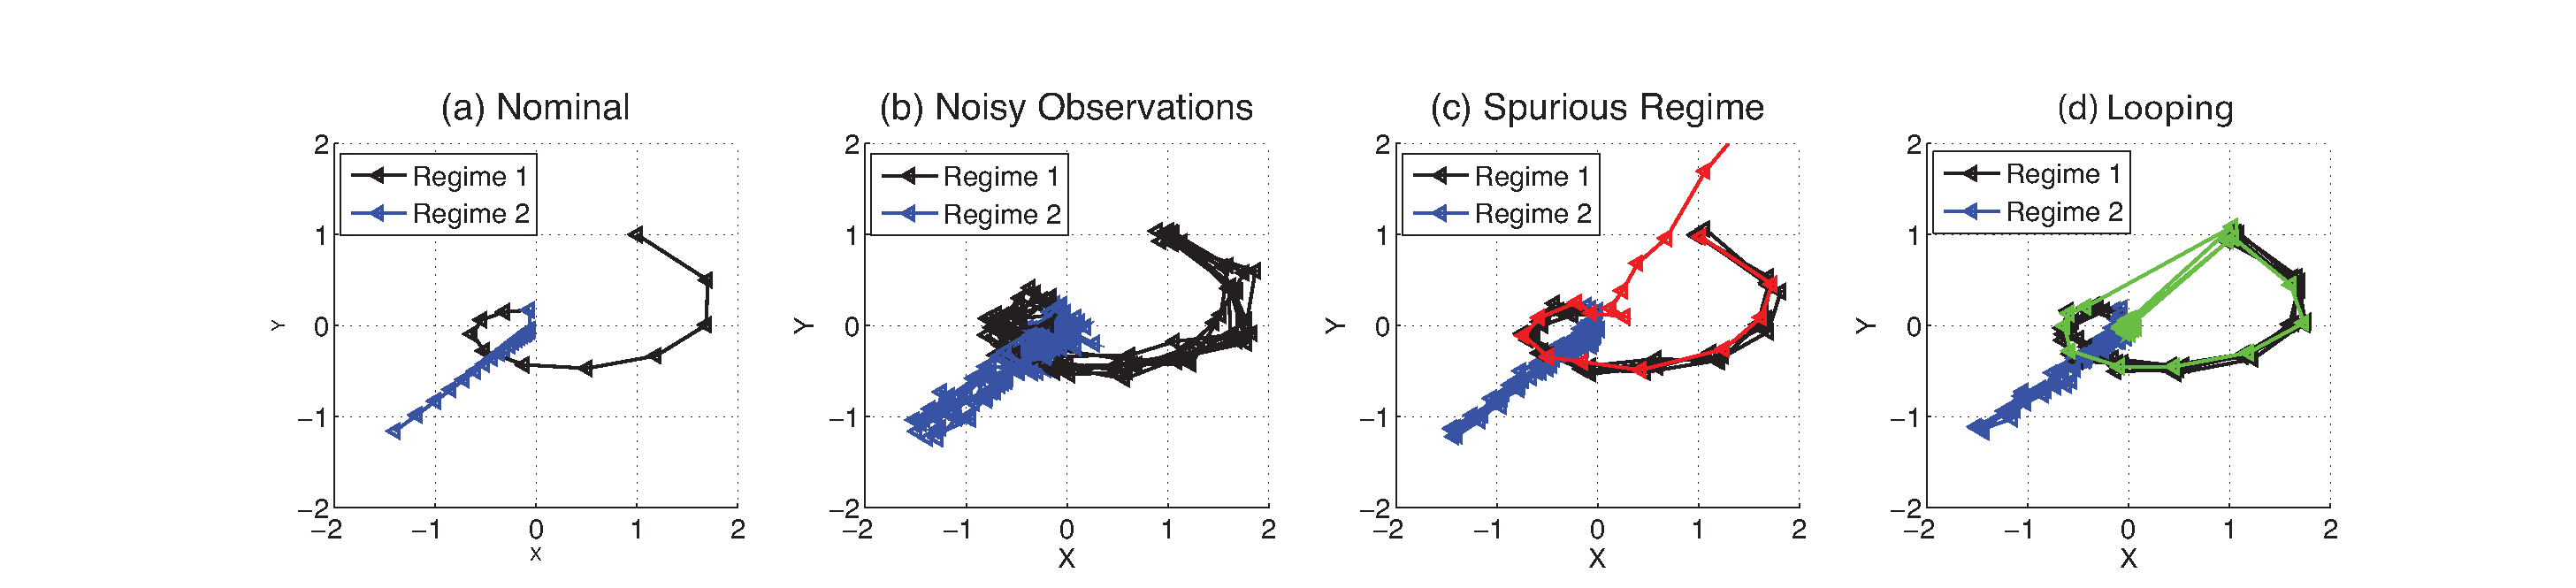
\includegraphics[width=\textwidth]{tsc-experiments/generated_data.pdf}
\caption{(a) Observations from a dynamical system with two regimes, (b) Observations corrupted with Gaussian Noise, (c) Observations corrupted with a spurious inserted regime (red), and (d) Observations corrupted with an inserted loop(green). \label{generated-data}}
% \vspace{-1em}
\end{figure*}

\begin{figure*}%[t]
\centering
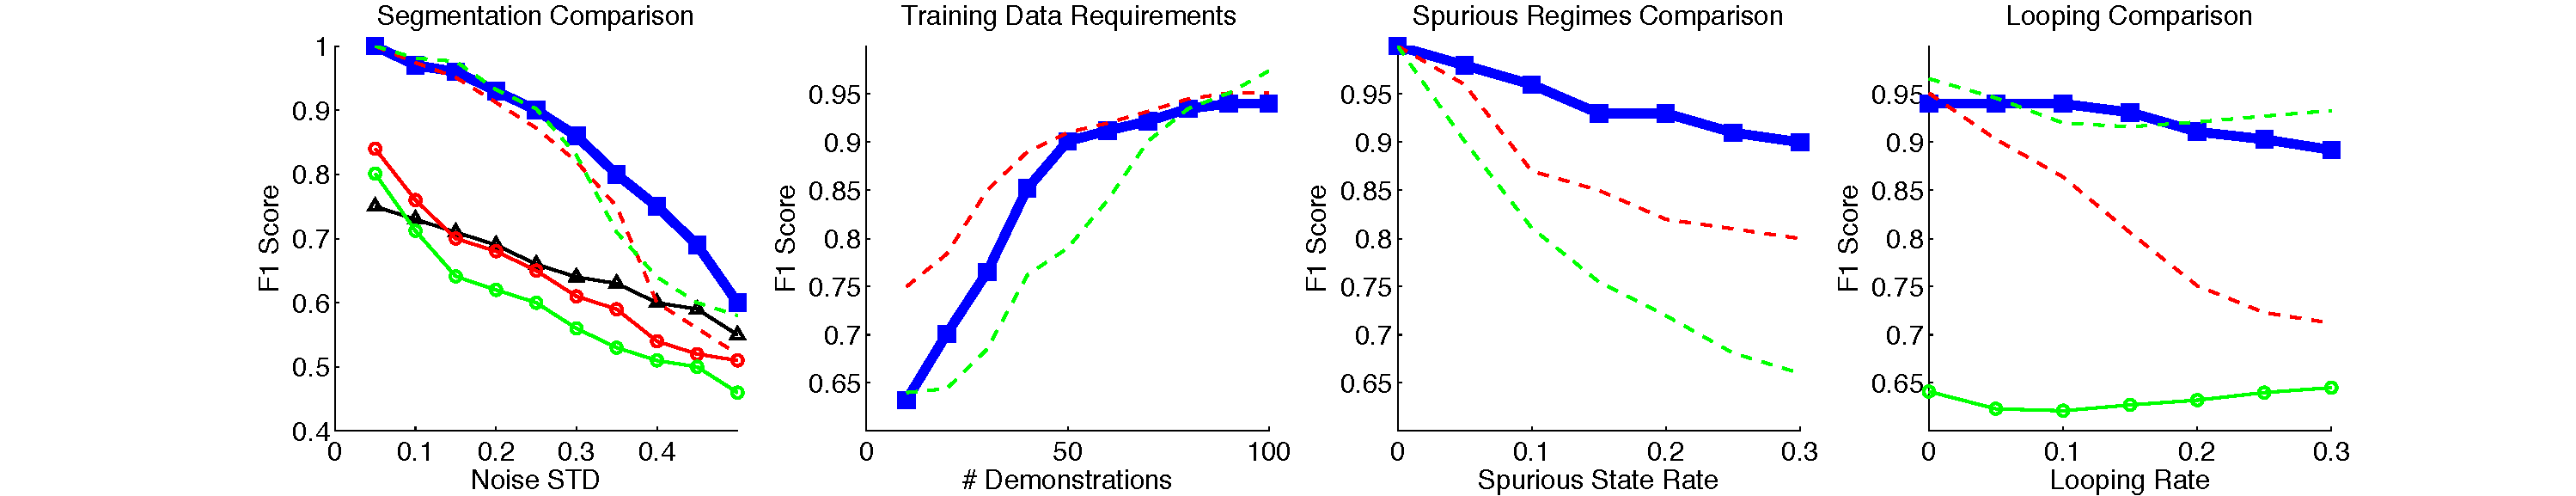
\includegraphics[width=\textwidth]{tsc-experiments/generated_comp.pdf}
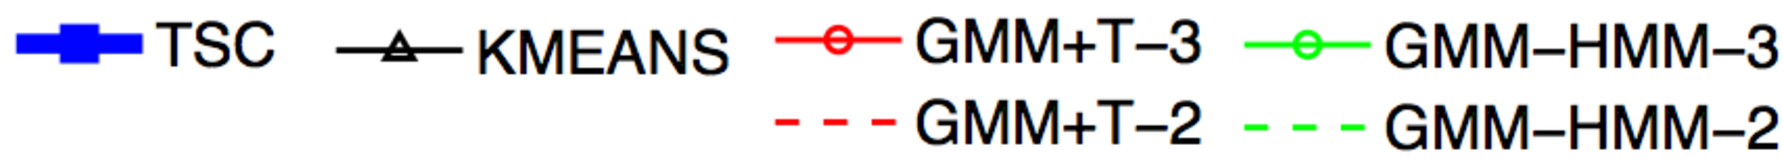
\includegraphics[width=0.6\textwidth]{tsc-experiments/toy_legend.pdf}
\caption{Accuracy as a function of noise: \tsc, K-Means, GMM+T (GMM with time), GMM+HMM (GMM with HMM). (a) The Dirichlet Process used in \tsc reduces sensitivity to parameter choice and is comparable to GMM techniques using the optimal parameter choice, (b) HMM based methods need more training data as they have to learn transitions, (c) \tsc clusters are robust to spurious regimes, and (d) \tsc clusters are robust to loops--without having to know the regimes in advance. \label{generated-comp}}
% 
\end{figure*}
\fi
